% Paquets généraux
\documentclass[a4paper,12pt,titlepage,twoside]{article}
\usepackage[T1]{fontenc}
\usepackage[utf8]{inputenc}
\usepackage[french]{babel}
\usepackage{subcaption}
\addto\captionsfrench{%
  \renewcommand{\tablename}{Tableau}%
}
\usepackage[gen]{eurosym}
%\usepackage[dvips]{graphicx}
\usepackage{minted}
\usepackage{fancyhdr}
\usepackage{pdfpages} 
\usepackage{multido}
\usepackage{hyperref}
\usepackage{textcomp}
\usepackage{schemabloc}
%\usepackage[bitstream-charter]{mathdesign}
\usepackage{array}
\newcolumntype{P}[1]{>{\centering\arraybackslash}p{#1}}
\usepackage[shortlabels]{enumitem}
\usepackage[framemethod=TikZ]{mdframed}

\newcommand{\id}{71}
\newcommand{\nom}{Théorie des mécanismes}
\newcommand{\sequence}{04}
\newcommand{\nomsequence}{Liaisons entre les solides}
\newcommand{\num}{02}
\newcommand{\type}{KH}
\newcommand{\descrip}{Liaisons équivalentes, hyperstatisme, liaisons en série et en parallèle, théorie des graphes}
\newcommand{\competences}{B2-12: Proposer une modélisation des liaisons avec leurs caractéristiques géométriques. \\ &  B2-13: Proposer un modèle cinématique paramétré à partir d'un système réel, d'une maquette numérique ou d'u \\ &  B2-17: Simplifier un modèle de mécanisme. \\ &  B2-18: Modifier un modèle pour le rendre isostatique. \\ &  C1-04: Proposer une démarche permettant d'obtenir une loi entrée-sortie géométrique.  \\ &  C2-05: Caractériser le mouvement d'un repère par rapport à un autre repère. \\ &  C2-06: Déterminer les relations entre les grandeurs géométriques ou cinématiques. }
\newcommand{\nbcomp}{7}
\newcommand{\systemes}{}
\newcommand{\systemesnum}{}
\newcommand{\systemessansaccent}{}
\newcommand{\ilot}{2}
\newcommand{\ilotstr}{02}
\newcommand{\dossierilot}{\detokenize{Ilot_02 }}

%\usepackage{style}
\usepackage{bodegraph}
\usepackage{rpcinematik}
\usepackage[locale = FR]{siunitx}
\usepackage{caption}
\newcommand{\institute}{Lycée Dorian}

\usepackage{listings}
\usepackage{fancyvrb}
\usepackage{color}
\usepackage{xcolor}
\usepackage{colortbl}
\usepackage{helvet}
\usepackage[frenchmath]{newtxsf} % for sans serif symbols
\renewcommand{\familydefault}{\sfdefault}
%\usepackage{amsfonts}
%\usepackage{amsmath}
%\usepackage{lmodern}
\usepackage{mathastext}
%\usepackage{xspace}
\usepackage{varioref}
\usepackage{tabularx}
%\usepackage{floatflt}
\usepackage{graphics}
\usepackage{wrapfig}
\usepackage{textcomp}
\usepackage{tikz,tkz-tab}
\usepackage[european resistor, european voltage, european current]{circuitikz}
\usepackage{wrapfig}
\usepackage{gensymb}
\usepackage[percent]{overpic}
\usetikzlibrary{babel}
\usepackage{ifthen}
\usepackage{cancel}
\usepackage{etoolbox}
\usepackage{multirow}
%\usepackage{boxedminipage}
\definecolor{gris25}{gray}{0.75}
\definecolor{bleu}{RGB}{18,33,98}
\definecolor{bleuf}{RGB}{42,94,171}
\definecolor{bleuc}{RGB}{231,239,247}
\definecolor{bleum}{RGB}{160,195,226}
\definecolor{rougef}{RGB}{185,18,27}
\definecolor{rougec}{RGB}{255,188,204}%255,230,231
\definecolor{vertf}{RGB}{103,126,82}
\definecolor{vertc}{RGB}{220,255,191}
\definecolor{forestgreen}{rgb}{0.13,0.54,0.13}
\definecolor{blcr}{rgb}{0.59,0.69,0.84}
\definecolor{blfr}{rgb}{0.32,0.51,0.75}
\definecolor{orfr}{rgb}{0.90,0.42,0.15}
\definecolor{orcr}{rgb}{0.90,0.65,0.50}
\definecolor{orangef}{rgb}{0.659,0.269,0.072}
\definecolor{orange}{rgb}{0.58,0.35,0.063}
\definecolor{orangec}{rgb}{0.43,0.32,0.25}
\definecolor{rcorrect}{rgb}{0.6,0,0}
\definecolor{sequence}{rgb}{0.75,0.75,0.75}
\definecolor{competences}{rgb}{0.61,0.73,0.35}
\definecolor{rose}{HTML}{ff00ff}
\definecolor{grisf}{HTML}{222222}
\definecolor{grisc}{HTML}{636363}
\definecolor{normal}{HTML}{4087c4}
\definecolor{info}{HTML}{5bc0de}
\definecolor{success}{RGB}{92,184,92}
\definecolor{warning}{RGB}{240,173,78}
\definecolor{danger}{RGB}{217,83,79}
\hypersetup{                    % parametrage des hyperliens
    colorlinks=true,                % colorise les liens
    breaklinks=true,                % permet les retours à la ligne pour les liens trop longs
    urlcolor= blfr,                 % couleur des hyperliens
    linkcolor= orange,                % couleur des liens internes aux documents (index, figures, tableaux, equations,...)
    citecolor= forestgreen                % couleur des liens vers les references bibliographiques
    }

\newcolumntype{M}[1]{>{\centering\arraybackslash}m{#1}}
\definecolor{codegreen}{rgb}{0,0.6,0}
\definecolor{codegray}{rgb}{0.5,0.5,0.5}
\definecolor{codepurple}{rgb}{0.58,0,0.82}
\definecolor{backcolour}{rgb}{0.95,0.95,0.92}

\lstdefinestyle{mystyle}{
    backgroundcolor=\color{backcolour},   
    commentstyle=\color{codegreen},
    keywordstyle=\color{magenta},
    numberstyle=\tiny\color{codegray},
    stringstyle=\color{codepurple},
    basicstyle=\ttfamily\footnotesize,
    breakatwhitespace=false,         
    breaklines=true,                 
    captionpos=b,                    
    keepspaces=true,                 
    numbers=left,                    
    numbersep=5pt,                  
    showspaces=false,                
    showstringspaces=false,
    showtabs=false,                  
    tabsize=2
}

\lstset{style=mystyle}

% Mise en page
\pagestyle{fancy}

\setlength{\hoffset}{-18pt}
\setlength{\oddsidemargin}{0pt} 	% Marge gauche sur pages impaire2s
\setlength{\evensidemargin}{0pt} 	% Marge gauche sur pages paires
\setlength{\marginparwidth}{00pt} 	% Largeur de note dans la marge
\setlength{\headwidth}{481pt} 	 	% Largeur de la zone de tête (17cm)
\setlength{\textwidth}{481pt} 	 	% Largeu\textbf{r de la zone de texte (17cm)
\setlength{\voffset}{-18pt} 		% Bon pour DOS
\setlength{\marginparsep}{7pt}	 	% Séparation de la marge
\setlength{\topmargin}{-30pt} 		% Pas de marge en haut
\setlength{\headheight}{55pt} 		% Haut de page
\setlength{\headsep}{20pt} 		% Entre le haut de page et le texte
\setlength{\footskip}{30pt} 		% Bas de\textbf{ page + séparation
\setlength{\textheight}{700pt} 		% Hauteur de l'icone zone de texte (25cm)
\setlength\fboxrule{1 pt}
\renewcommand{\baselinestretch}{1}
\setcounter{tocdepth}{1}
\newcommand{\cadre}[2]
{\fbox{
  \begin{minipage}{#1\linewidth}
   \begin{center}
    #2\\
   \end{center}
  \end{minipage}
 }
}

\newcommand{\repon}[1]
{
~\ \\
\begin{tabular}{|m{\linewidth}|}
 \hline
\multido{}{#1}{\\ \hline}
\end{tabular}
}


\newcommand{\objectif}[1]{
\mdfsetup{%
frametitle={%
\tikz[baseline=(current bounding box.east),outer sep=0pt]
\node[anchor=east,rectangle,fill=bleum]
{\strut Objectif~};}}
\mdfsetup{innertopmargin=10pt,linecolor=bleum,%
linewidth=2pt,topline=true,%
frametitleaboveskip=\dimexpr-\ht\strutbox\relax
}
\begin{mdframed}[]\relax%
#1
\end{mdframed}}


\newcounter{num_quest} \setcounter{num_quest}{0}
\newcounter{num_rep} \setcounter{num_rep}{0}
\newcounter{num_cor} \setcounter{num_cor}{0}

\newcommand{\feuilleDR}[1]{
	\begin{tikzpicture}
		\draw[gray!30](0,0)grid[step=0.5cm](\linewidth,#1);
	\end{tikzpicture}
}

%\newcommand{\question}[1]{\refstepcounter{num_quest}\par
%~\ \\ \parbox[t][][t]{0.15\linewidth}{\textbf{Question \arabic{num_quest}}}\parbox[t][][t]{0.85\linewidth}{#1\label{q\the\value{num_quest}}}\par
%}

\newcommand{\question}[1]{\refstepcounter{num_quest}\par
~\ \\ \textbf{Question \arabic{num_quest} : }#1\label{q\the\value{num_quest}}\par
}

\newcommand{\posetafigure}[3]{
\begin{figure}[ht!]
 \begin{center}
  \includegraphics[width=#2\linewidth]{img/#1}
 \end{center}
 \caption{\label{#1} #3}
\end{figure}}

\newcommand{\goforum}{
\begin{figure}

\end{figure}
\begin{center}
 
\includegraphics[width=0.7\linewidth]{../../../img/go_forum}
\end{center}
\label{go_forum}
\caption{J'pète les plombs}
\end{figure}}

\newcommand{\reponse}[4][1]
{\noindent
\parbox{\textwidth}{
\rule{\linewidth}{.5pt}\\
\textbf{Question\ifthenelse{#1>1}{s}{} \multido{}{#1}{%
\refstepcounter{num_rep}\ref{q\the\value{num_rep}} }:} ~\ \\
\ifdef{\public}{#3 \ifthenelse{#2>0}{~\ \\ 	\feuilleDR{#2}}}{#4}
}}

\newcommand{\cor}
{\refstepcounter{num_cor}
\noindent
\rule{\linewidth}{.5pt}
\textbf{Question \arabic{num_cor}:} \\
}

\newcommand{\finsujet}
{
    \begin{center}
    \Large{FIN}
    \end{center}

    \cleardoublepage

    \ifdef{\public}{\pagestyle{docreponse}}{\pagestyle{correction}}

    \ifdef{\public}{
        \begin{tikzpicture} 
            \draw (0,0) rectangle (2,2);
            \draw (0,0) -- (2,2);
            \draw (1.5,0.5) node {\large 20};
            \draw (2.5,0) rectangle (16,2);
            \draw (4.5,1.7) node {\large Commentaires:};
        \end{tikzpicture}
    }
    ~\ \\
}


%\newcommand{\repcarre}[2]
%{
%~\ \\
%\begin{tikzpicture}
%\draw [fill=white] (0,0) rectangle +(\linewidth,#1);
%\node[align=left] at (1.1,#2-0.3) {\textbf{Question #1:}};
%\end{tikzpicture}
%}

\newcommand{\titre}[1]
{\begin{center}
\cadre{0.8}{\huge #1} 
\end{center}
}


%Définition des torseurs :
\newcommand{\torseur}[2]{\left\{\mathcal{#1}_{#2} \right\}}
\newcommand{\torseurh}[3]{\left\{\genfrac{}{}{0pt}{0}{#1}{#2}\right\}_{#3}}
\newcommand{\torseurv}[8]{\left\{
\begin{matrix}
#1 & #4 \\ #2 & #5 \\ #3 &#6
\end{matrix}
\right\}_{{#7},{#8}}}

%Définition des torseurs :
%\newcommand{\torseur}[2]{\left \{\mbox{\relsize{2}{$\mathcal {#1}$}\relsize{-2}}\phantom{}_{\mbox{\scriptsize $#2$}} \right \}}
%\newcommand{\torseurh}[3]{\left\{\genfrac{}{}{0pt}{0}{#1}{#2}\right\}_{#3}}
%\newcommand{\torseurv}[8]{
%\left\{\begin{array}{@{}c|c@{}} #1 & #4 \\ #2 & #5 \\ #3 & #6 \end{array} \right\}_{#7,#8}
%}
\newcommand{\derivee}[2]{\left.\dfrac{\d #1}{\d t}\right|_{#2}}
\newcommand{\tripleint}{\int\!\!\!\!\!\int\!\!\!\!\!\int}

% Notation cinématique et statique
\newcommand{\cinematique}[2]{\mbox{#1}/\mbox{#2}}
\newcommand{\statique}[2]{\mbox{#1}\rightarrow\mbox{#2}}
\newcommand{\moment}[3]{\vv {#1}_{\scriptsize{#3}}(#2)}
\newcommand{\resultante}[2]{\vv {#1}_{\scriptsize{#2}}}


%Commande de base
\newcommand{\jo}{\left(j\omega\right)} % j \omega dans l'analyse fréquentielle
\newcommand{\tl}{\xrightarrow{\mathcal{L}}} % transformée de laplace sur fleche
\newcommand{\tli}{\xrightarrow{\mathcal{L}^{-1}}} % transformée inverse de laplace sur fleche
\renewcommand{\d}[1][]{\mathrm{d#1}}
\newcommand{\dd}[1][]{\mathrm{d#1}}
\newcommand{\vect}[2]{{#1}\wedge{#2}}
\newcommand{\base}[3]{(\vec #1,\vec #2,\vec #3)}
\newcommand{\vectbase}[4]{{\vphantom{\left| \begin{matrix}
#1\\#2\\#3 \end{matrix} \right|}}_{#4}{\left| \begin{matrix}
#1\\#2\\#3 \end{matrix} \right.}}
%Pour avoir les paragraphes sous la forme I, II, III
\renewcommand{\thesection}{\Roman{section}}
\setcounter{secnumdepth}{3}
\renewcommand{\Frlabelitemii}{$\bullet$}

% En tête et pied de page
\lhead{\nom}
\rhead{
\includegraphics[width=2cm]{../../../img/logo}}
\lfoot{\auteurun,\ \auteurdeux}
\cfoot{Page \thepage}

\fancypagestyle{docreponse}{%
  \fancyhf{}
  \fancyhead[LO]{NOM Prénom: .............................}
  \rhead{
\includegraphics[width=2cm]{../../../img/logo}\hspace{2pt}}
  \ifdef{\auteurdeux}{\lfoot{\auteurun,\ \auteurdeux}}{\lfoot{\auteurun}}
  \rfoot{\nom}
  \lfoot{Document réponse}
  \cfoot{Page \thepage}
   }

\fancypagestyle{correction}{%
  \fancyhf{}
  \lhead{\colorbox{danger}{\begin{minipage}{0.65\paperwidth} \textcolor{white}{\textbf{Correction}} \end{minipage}} }
  \rhead{
\includegraphics[width=2cm]{../../../img/logo}}
  \lfoot{Renaud Costadoat, Françoise Puig}
  \rfoot{\colorbox{danger}{\begin{minipage}{0.4\paperwidth} \begin{flushright}\textcolor{white}{\textbf{Correction}}\end{flushright} \end{minipage}} }}

\fancypagestyle{correctioninfo}{%
  \fancyhf{}
  \lhead{\colorbox{danger}{\begin{minipage}{0.65\paperwidth} \textcolor{white}{\textbf{Correction}} \end{minipage}} }
  \rhead{
\includegraphics[width=2cm]{../../../img/logo}}
  \lfoot{Renaud Costadoat, Juliette Genzmer}
  \rfoot{\colorbox{danger}{\begin{minipage}{0.6\paperwidth} \begin{flushright}\textcolor{white}{\textbf{Correction}}\end{flushright} \end{minipage}} }}

\renewcommand{\footrulewidth}{0.4pt}

\usepackage{eso-pic}
\newcommand{\BackgroundPic}{%
\put(0,0){%
\parbox[b][\paperheight]{\paperwidth}{%
\vfill
\begin{center}
\hspace{0.5cm}\vspace{0.5cm}

\includegraphics[width=\paperwidth,height=\paperheight,%
keepaspectratio]{../../../img/fond3}%
\end{center}
\vfill
}}}

\newcommand{\BackgroundPicdeux}{%
\put(25,-30){%
\parbox[b][\paperheight]{\paperwidth}{%
\vfill
\begin{center}
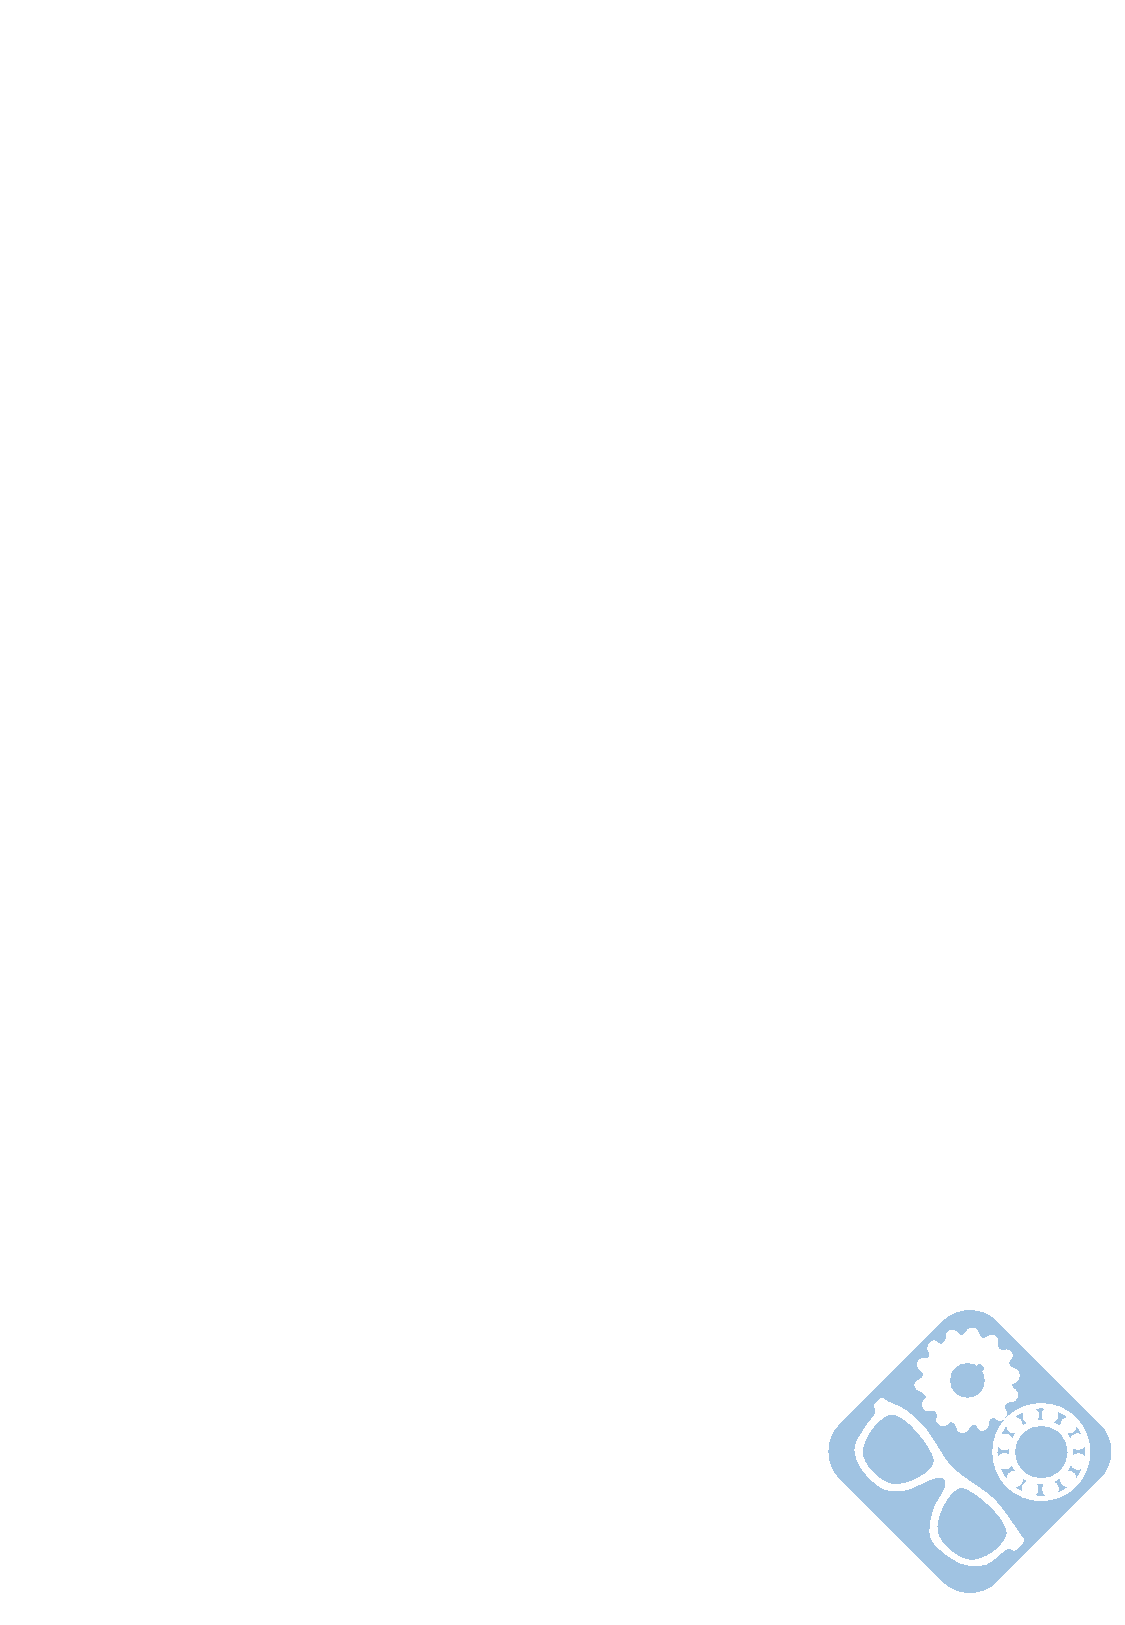
\includegraphics[width=\paperwidth,height=\paperheight,%
keepaspectratio]{../../../img/fond4}%
\end{center}
\vfill
}}}

\begin{document}

\pagestyle{empty}

\AddToShipoutPicture*{\BackgroundPic}


\includegraphics[width=2cm]{../../../img/logo}

\Huge{DS \numero - \sujet}

\vspace{1cm}

\ifdef{\prive}{\begin{center}\colorbox{danger}{\Huge{Avec Correction}}\end{center}}{}

\begin{center}
\centering\huge{PTSI}
\end{center}

\vspace{2cm}


\begin{center}
\centering\Large{\jour}
\end{center}

\vspace{2cm}

\normalsize

\tableofcontents

\newpage

\AddToShipoutPicture{\BackgroundPicdeux}

\pagestyle{fancy}

\begin{center}
\Huge \sujet
\end{center}


\normalsize


La société Commercy Robotique, implantée en région Grand Est, est spécialisée dans l’intégration de solutions robotisées auprès des PME françaises. La grande partie de ses activités est historiquement centrée sur le soudage.

Cette entreprise propose en particulier à ses clients des cellules de soudage robotisé standards compactes, fiables et faciles d’utilisation. 
Elles s’intègrent facilement dans n’importe quel atelier et permettent un rapide retour sur investissement.

Grâce à leur conception innovante et à leur flexibilité, ces cellules sont une alternative intéressante aux machines spéciales de soudage automatique.

\begin{figure}[!h]
\centering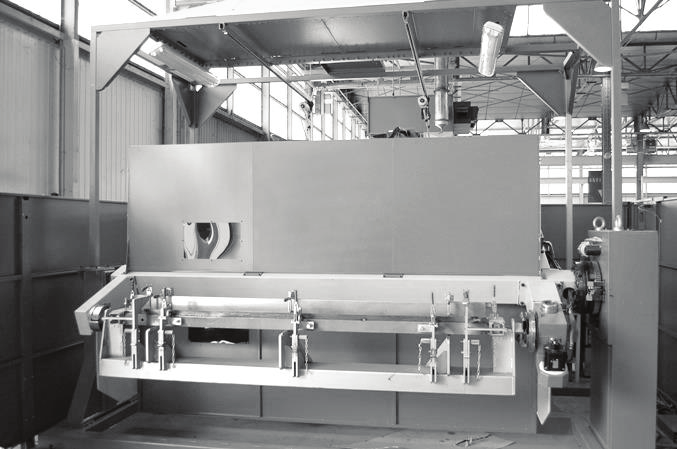
\includegraphics[width=0.8\linewidth]{img/fig01}
 \caption{Photo d'un robot de soudage en situation industrielle}
 \label{img01}
\end{figure}

\section*{Cahier des Charges Fonctionnel partiel}

\subsection*{Présentation du problème}

\paragraph{Le contexte}

Afin de répondre au mieux aux besoins de ses clients, l’entreprise propose une gamme de robots de soudage avec différentes architectures capables de recevoir des pièces à souder de tailles et de masses variées. Dans le cadre du travail qui est demandé ici, il s’agit de
diminuer la capacité de charge d’un robot existant, afin de se positionner commercialement sur le marché des pièces légères.

\paragraph{Le poste de soudage}

Le \og poste de soudage robotisé \fg\ est une machine comprenant :
\begin{itemize}
 \item un robot industriel de type bras articulé et équipé à son extrémité du \og dispositif de soudage \fg\ selon le procédé de soudage utilisé,
 \item un poste de chargement/déchargement.
\end{itemize}

Le poste de chargement/déchargement est constitué d’une broche horizontale comprenant deux \og outillages de soudage \fg\ identiques séparés par une plaque de protection verticale. Chaque \og outillage de soudage \fg\ permet de maintenir en position la pièce à souder. Ces outillages sont également pilotables en rotation autour d’un axe
horizontal.

\begin{figure}[!h]
\centering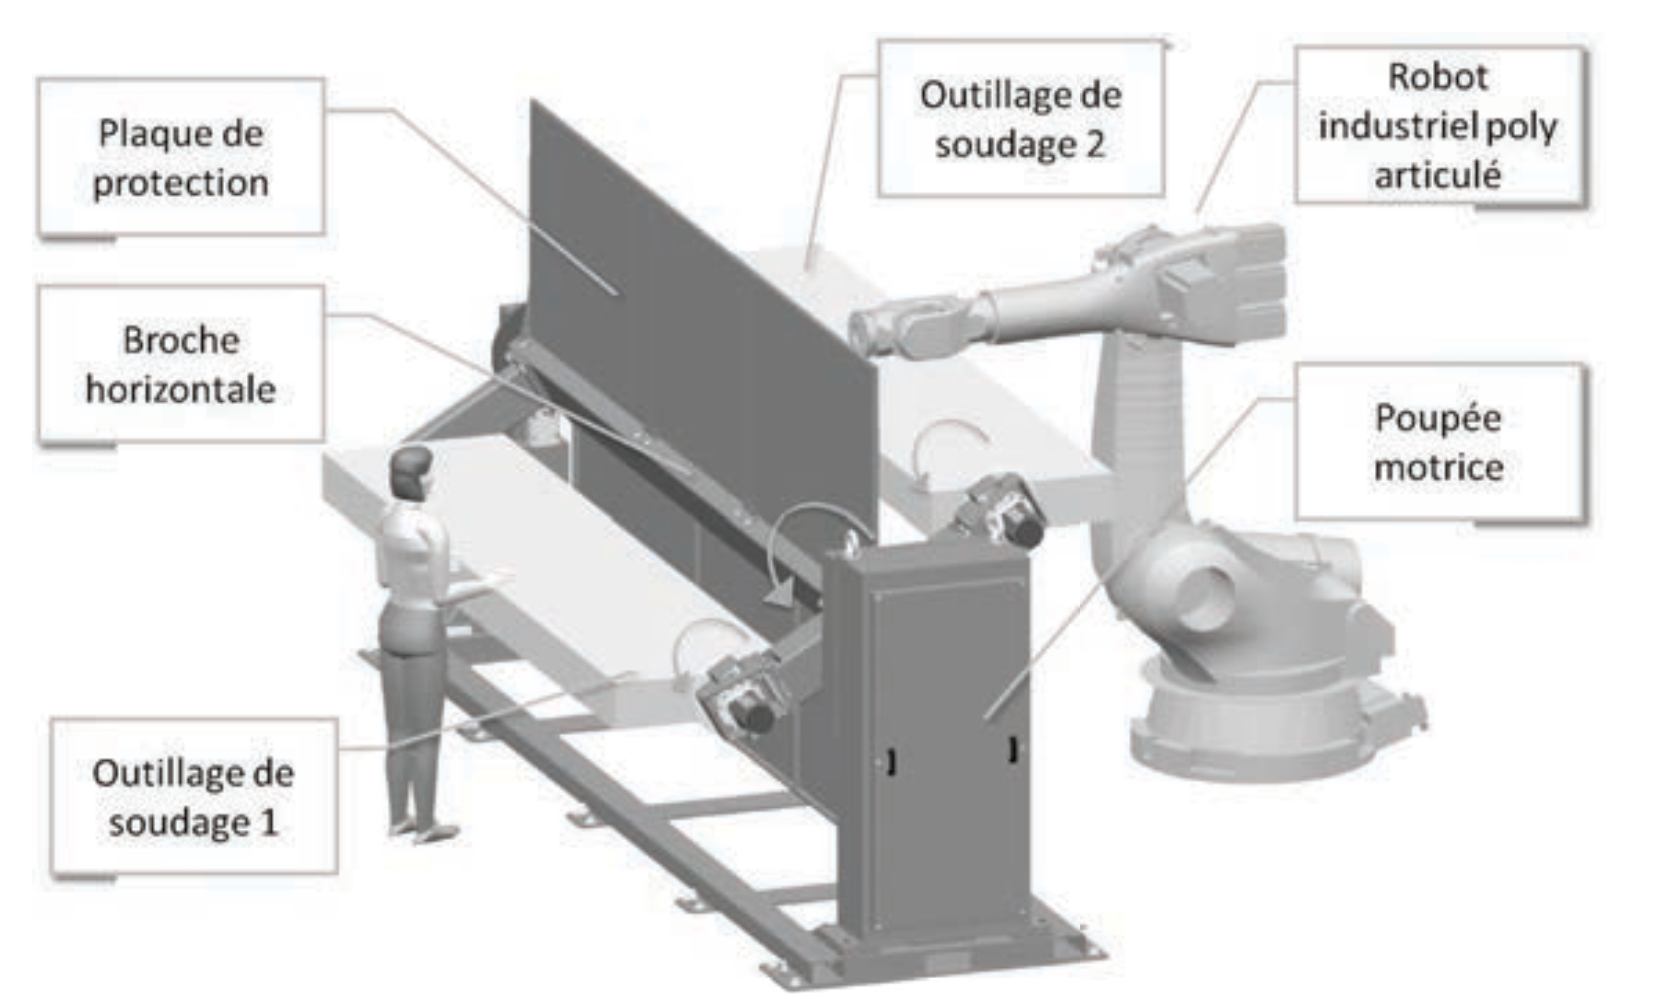
\includegraphics[width=0.7\linewidth]{img/fig02}
 \caption{Les différents éléments d'un robot de soudage}
 \label{img02}
\end{figure}

\vspace{-1cm}

\paragraph{Principe de fonctionnement du soudage}

\begin{figure}[!h]
\begin{minipage}{0.49\linewidth}
Pendant que le bras articulé soude la pièce installée sur l’outillage
de soudage 2, l’opérateur, protégé des projections et rayonnements par la plaque verticale, décharge de l’outillage de soudage 1 une pièce qui vient d’être soudée.

Une fois la pièce déchargée, il en installe une autre à souder.

Quand cette opération est terminée par l’opérateur et que le
robot a terminé ses opérations de soudage, la poupée motrice
tourne la broche de 180° et permute donc les deux assemblages
de soudage.

Le bras robotisé peut souder la nouvelle pièce pendant que l’opérateur répète ses manipulations de déchargement/chargement.
\end{minipage}\hfill
\begin{minipage}{0.5\linewidth}
\centering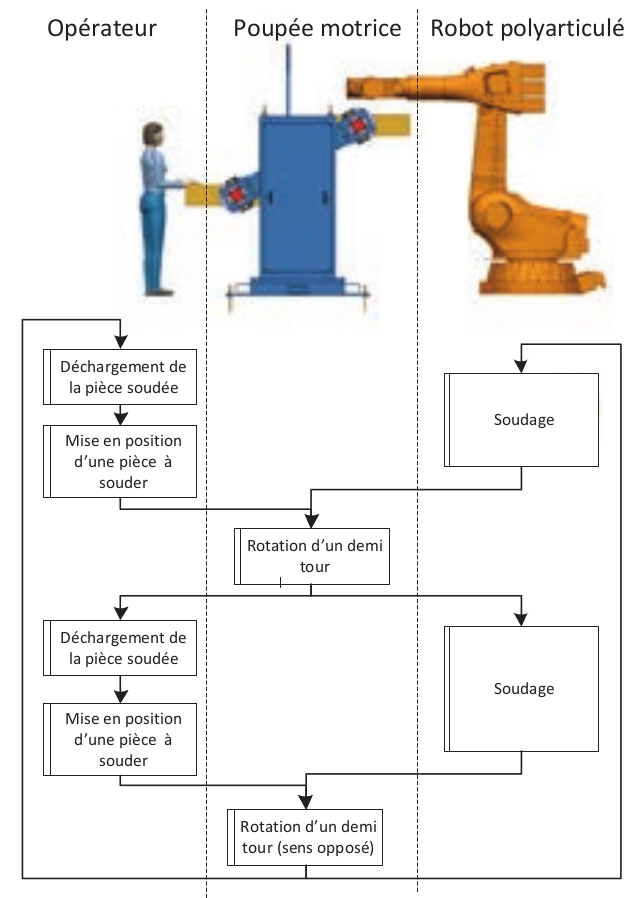
\includegraphics[width=0.95\linewidth]{img/fig03}
 \caption{Séquencement des opérations}
 \label{img03}
\end{minipage}
\end{figure}

En phase de fonctionnement normal (production) les principales exigences sont énoncées dans le diagramme ci-dessous (Figure \ref{img04}). En phase de réglage de la machine, la motorisation et les organes de sécurité doivent permettre un fonctionnement avec un seul outillage et une seule pièce installée.

\begin{figure}[!h]
\centering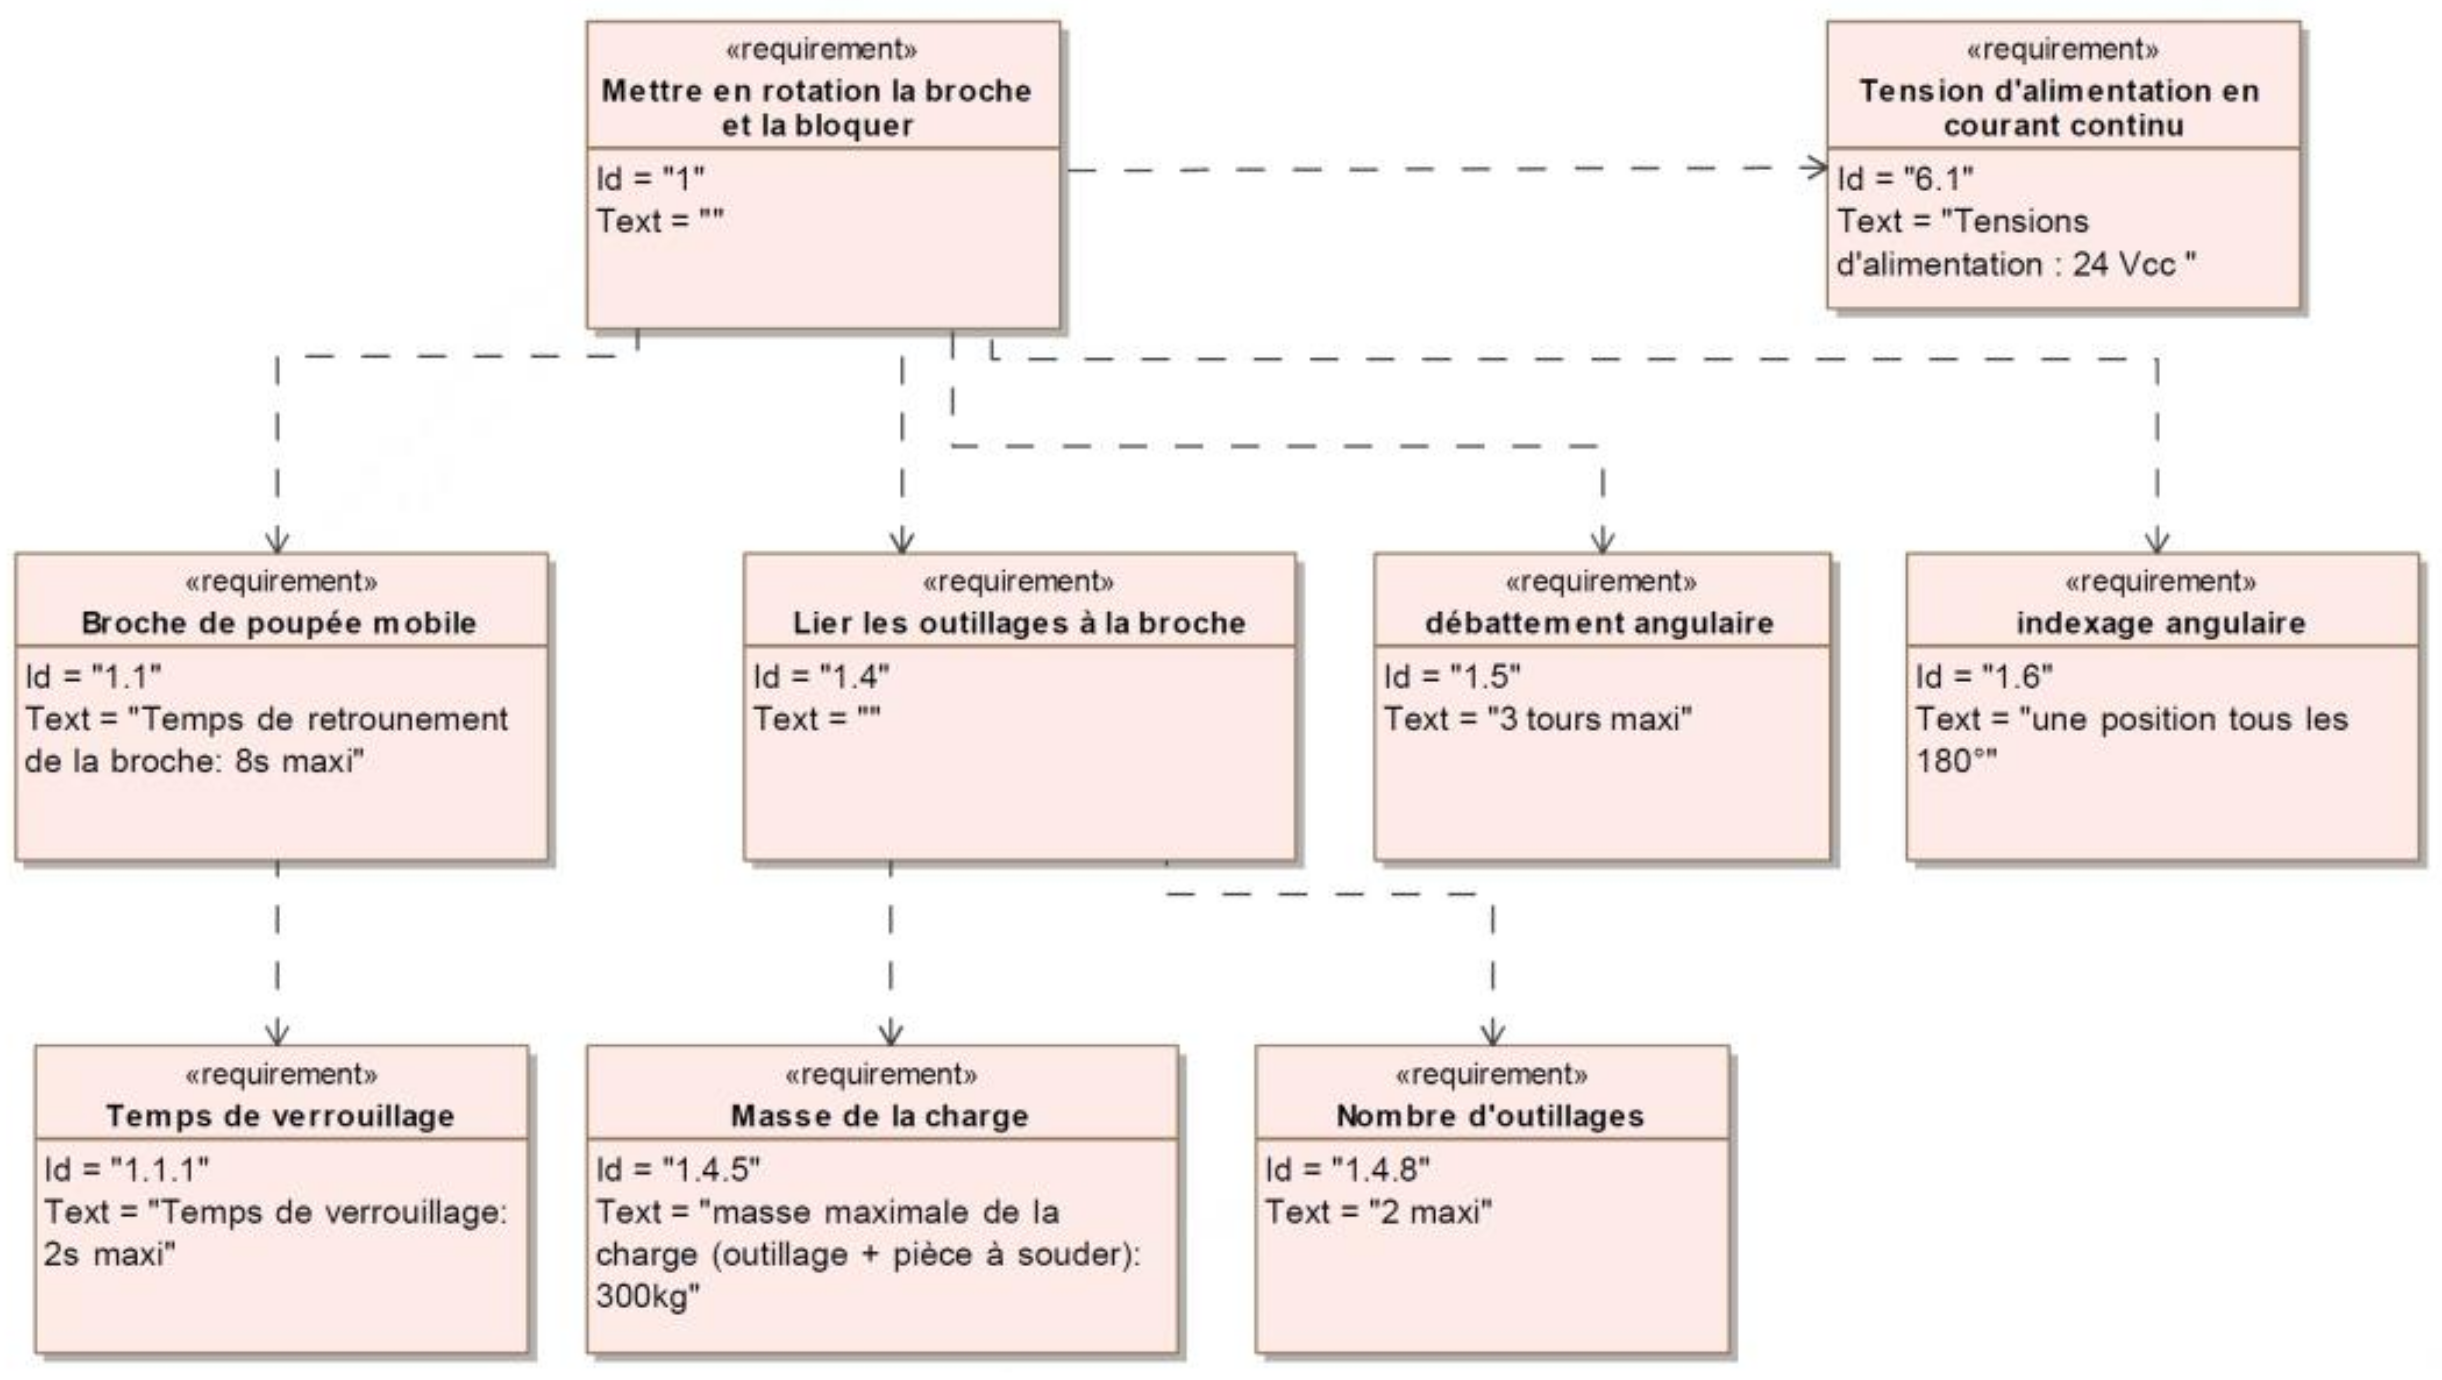
\includegraphics[width=0.9\linewidth]{img/fig04}
 \caption{Extraits du diagramme des exigences en phase de fonctionnement normal}
 \label{img04}
\end{figure}

\paragraph{Objet de l’étude}

Le mécanisme étudié est limité ici à une sous-partie du robot : le système de verrouillage de la poupée motrice.

\begin{figure}[!h]
\centering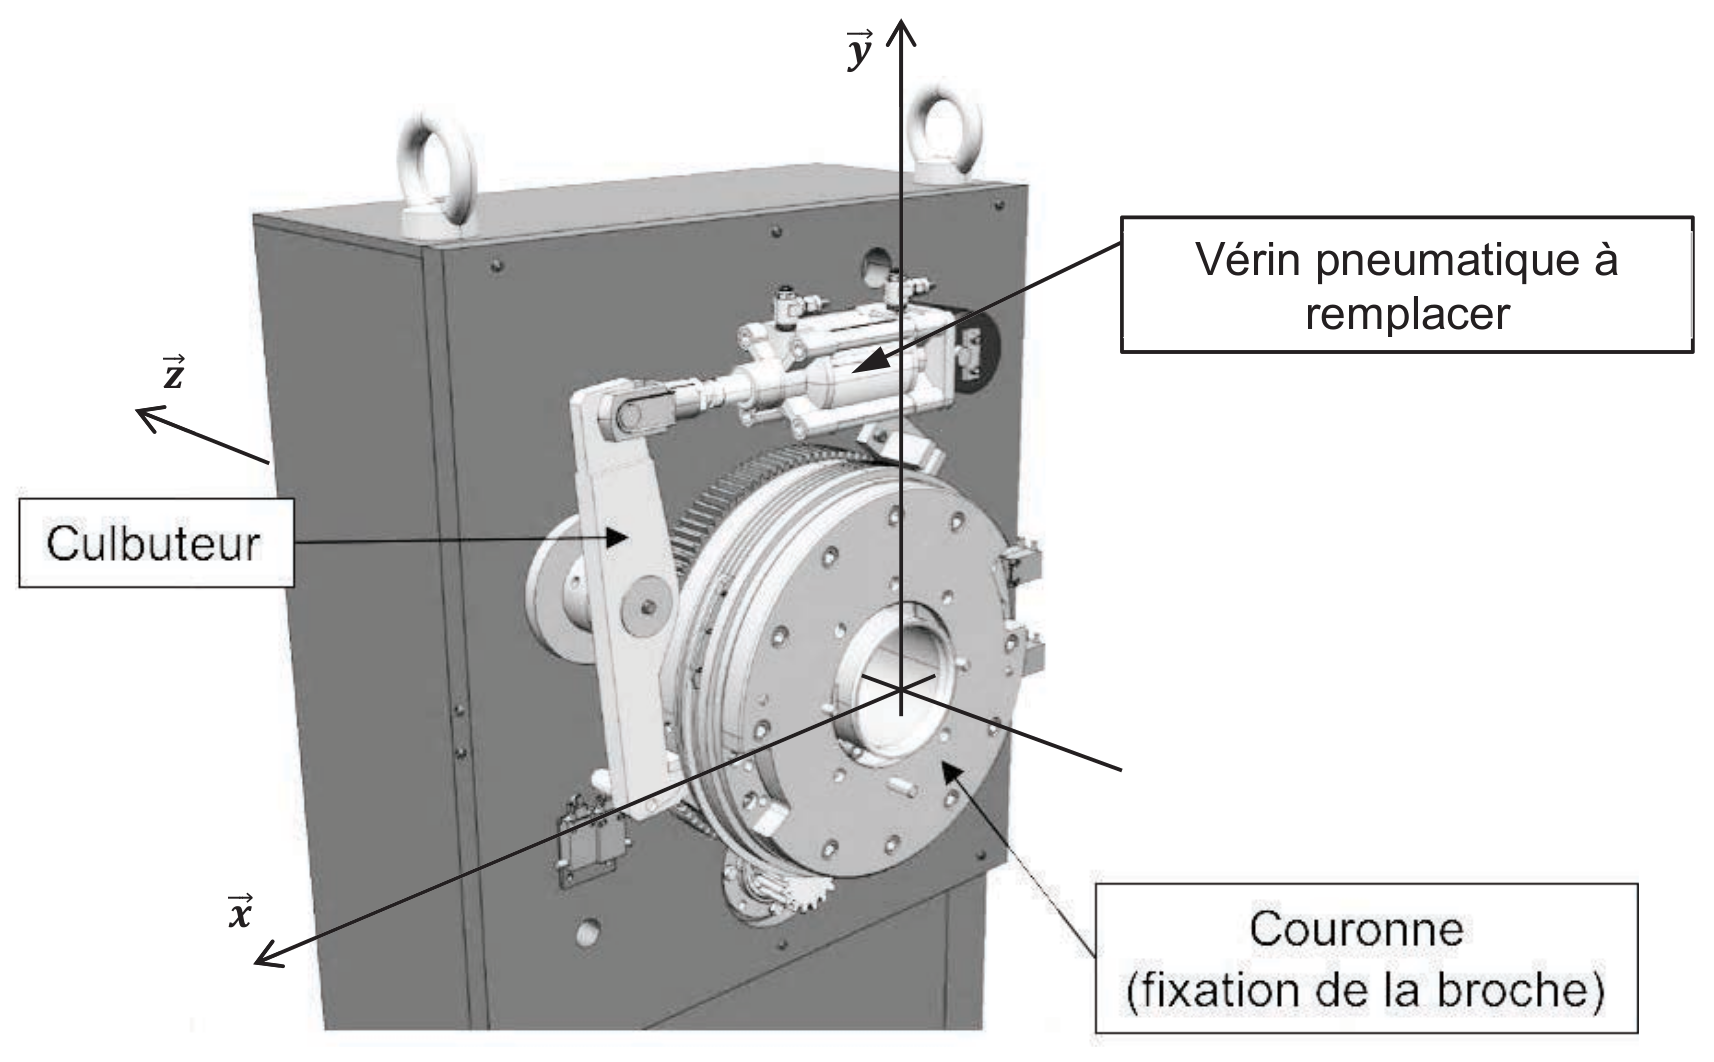
\includegraphics[width=0.6\linewidth]{img/fig05}
 \caption{Vue de la poupée motrice et de son système de verrouillage}
 \label{img05}
\end{figure}

\begin{figure}[!h]
\begin{minipage}{0.55\linewidth}
La poupée motrice permet le maintien et la rotation d’un demi-tour de la broche.

Celle-ci, montée sur la couronne 6 est maintenue par un assemblage vissé. Un système de verrouillage {3, 4, 5, 8} permet de bloquer la rotation de la broche. Lorsqu’elle est libérée, elle effectue un demi-tour sur elle-même grâce à un motoréducteur non-représenté.

Sur le système actuel, le vérin de verrouillage {3,4} est un vérin pneumatique. Dans le cadre de cette étude, il est demandé de le remplacer par un vérin électrique, de plus faible capacité et offrant plus de possibilités de pilotage.
\end{minipage}\hfill
\begin{minipage}{0.42\linewidth}
\centering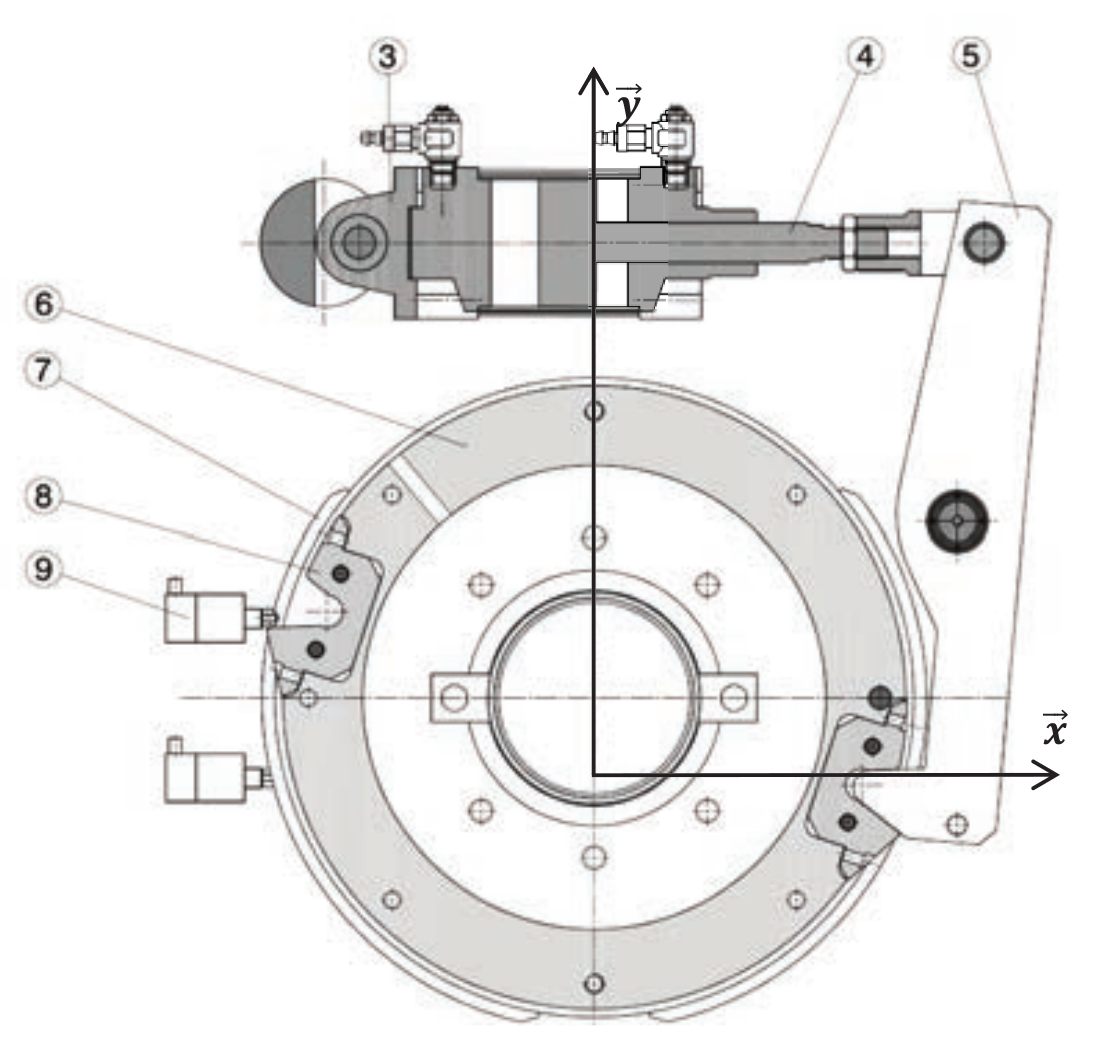
\includegraphics[width=0.95\linewidth]{img/fig06}
 \caption{Coupe du système de verrouillage}
 \label{img06}
\end{minipage}
\end{figure}

De  plus,  les  vés  de  verrouillage  8,  à  contact  direct  avec  le  levier  5,  subissent  une  usure  prématurée  dans  la  version  actuelle.  Dans  le  cadre  de  cette  étude,  il  est  demandé  de  les  remplacer par des vés à galets.

\begin{figure}[!h]
\centering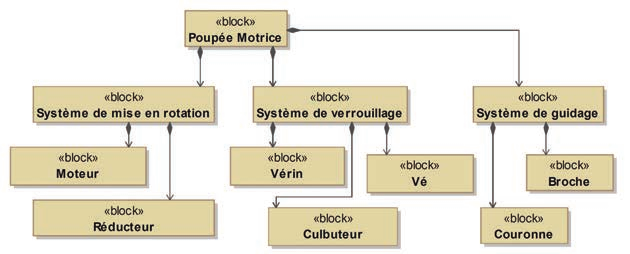
\includegraphics[width=0.6\linewidth]{img/fig07}
 \caption{Diagramme de blocs de la poupée motrice}
 \label{img07}
\end{figure}

\newpage
\paragraph{Travail demandé}

Ce  sujet  comporte  cinq  parties  indépendantes,  elles-mêmes  constituées  de  plusieurs questions qui peuvent être traitées séparément :
\begin{itemize}
 \item la  Partie  I  (durée  conseillée  20  min)  concerne l’étude de  la  course  du  nouveau  vérin électrique,
 \item la Partie II (durée conseillée 1h10) concerne la détermination des efforts mis en jeux dans le système de verrouillage,
 \item la Partie III (durée conseillée 30 min) concerne le choix d’un vérin électrique,
 \item la  Partie  IV  (durée  conseillée  1h30)  se  concentre  sur  la  représentation  des  solutions technologiques retenues pour l’implantation du nouveau vérin électrique et des galets.
\end{itemize}

Une lecture préalable du sujet complet est vivement conseillée (durée indicative 30 min).
 
\paragraph{Applications numériques}

Dans le domaine des Sciences Industrielles, le fait de savoir calculer et analyser les valeurs des grandeurs utiles au dimensionnement est aussi important que celui de savoir déterminer leurs expressions littérales. C’est pourquoi, une attention toute particulière sera accordée à la réalisation des applications numériques. Pour réaliser celles-ci sans l’usage d’une calculatrice, le candidat pourra faire des approximations de bon sens, qui conduiront éventuellement à une erreur relative de quelques pourcents sur le résultat final, tolérée par le correcteur.

\section{Détermination de la course du vérin}

\paragraph{Objectif:}

Déterminer la course minimale que doit avoir le vérin en fonction de la géométrie imposée de différentes pièces standardisées et du débattement du système de verrouillage.

Sur le document réponse est représenté schématiquement le système de verrouillage en position verrouillée à l'échelle 1/3. On y distingue:
\begin{itemize}
 \item l'articulation du vérin avec le bâti en E,
 \item l'articulation entre le vérin et le culbuteur en $D_0$,
 \item l'articulation entre le culbuteur et le bâti en C,
 \item la couronne, guidée en rotation par rapport au bâti en O,
 \item les deux galets liés à la couronne,
 \item les points de contact $A'_0$ et $A''_0$ entre le culbuteur et les deux galets,
 \item le centre $B_0$ du rayon de l'extrémité du culbuteur.
\end{itemize}

En position verrouillée, les différents points du mécanisme sont indicés \og 0 \fg.

En position déverrouillée, les différents points du mécanisme sont indicés \og 1 \fg.

Pendant la rotation de la couronne, afin d'éviter toute collision avec le culbuteur, celui-ci doit totalement être dégagé de la couronne et des galets avec une marge de 10mm. Cet espace de dégagement est représenté sur le document réponse par un arc de cercle de trait mixte fin.

\question{Tracer le point $B_1$, centre du rayon de l'extrémité du culbuteur, dans la position déverrouillée.

Tracer le point $D_1$, centre de l'articulation entre la tige du vérin et le culbuteur, dans la position déverrouillée.}

\question{Déduire de la question précédente les longueurs maximale et minimale du vérin, $L_{max}$ et $L_{min}$.

En déduire, la course minimale du vérin $C_{min}$.}

\section{Détermination des efforts mis en jeux dans le système de verrouillage}

\paragraph{Objectifs}

Identifier les cas de charges les plus défavorables, déterminer le couple de verrouillage et les efforts qui en résultent sur les galets, le culbuteur et le vérin.

\paragraph{Détermination du couple de verrouillage}

La broche est équipée de deux postes contenant chacun un outillage de soudage ($OS_1$ et $OS_2$). Chaque outillage peut accueillir une pièce à souder ($PS_1$ et $PS_2$). Se référer à l’annexe A, page A1/9.

Données:
\begin{itemize}
 \item La masse maximale d’un outillage de soudage est : $M_{os\_max}=  100kg$,
 \item La masse maximale d’une pièce à souder est : $M_{PS\_max}=200kg$,
 \item L’excentration des axes de rotation des outillages est : $e=750mm$,
 \item L’angle définissant la position de verrouillage est : $\alpha=30°$ modulo $\pi$ par rapport à l’axe de la broche,
 \item L’accélération de la pesanteur : $g\approx 10ms^{-2}$,
 \item On prendra : $cos(30°)=sin(60°)\approx 0,87$ et $cos(60°)=sin(30°)=0,5$.
\end{itemize}

\paragraph{Hypothèses}

Les outillages de soudage et les pièces à souder sont montés de telle manière que leurs centres de gravité sont respectivement sur les axes $(O_1,\vec{z})$ et $(O_2,\vec{z})$.

Le centre de gravité de la broche vide (sans OS) est sur l’axe $(O,\vec{z})$.

\paragraph{Notations :}

On note $C_{Verrouillage}$ la composante sur $(O,\vec{z})$ du moment exercé par l’ensemble $E=\left\{broche,\ OS_1,\ OS_2,\ PS_1,\ PS_2\right\}$ sur la couronne 6, et $\|\vec{P}_1\|$ et $\|\vec{P}_2\|$ les poids des outillages et des pièces à souder.

\question{Après avoir isolé E, et fait un bilan des actions mécaniques qu'il subit, donner l'expression du couple de verrouillage $C_{Verrouillage}$ en fonction de $\|\vec{P}_1\|$, $\|\vec{P}_2\|$ et de caractéristiques géométriques du système.}

~\

Pendant le fonctionnement et le réglage du robot, la broche doit toujours pouvoir tourner et être verrouillée. Différents cas peuvent se présenter :
\begin{itemize}
 \item aucun outillage monté,
 \item un outillage monté,
 \item deux outillages montés, mais sans pièces à souder,
 \item deux outillages montés et une seule pièce à souder installée,
 \item ...
\end{itemize}

Les principales combinaisons sont répertoriées dans le cahier réponse. Chaque combinaison sollicite différemment le système de verrouillage.

\question{Compléter le tableau du cahier réponse en précisant les normes des poids $\vec{P}_1$, $\vec{P}_2$ et l’intensité et le sens du couple de verrouillage $C_{Verrouillage}$ (trois chiffres significatifs).}

\question{En déduire l’intensité maximale du couple de verrouillage dans le sens positif et négatif.}

\question{Dans quelle situation de vie du robot le système de verrouillage est-il potentiellement le plus sollicité : fonctionnement normal (production) ou en phase de réglage ? Justifiez.}

\subsection{Détermination des efforts dans les galets}

Le paramétrage du contact entre le culbuteur et les galets est donné en annexe B, page A2/9.

\paragraph{Notations :}

On note TRS, le théorème de la résultante statique et TMS, le théorème du moment statique.

On note $\left\|\overrightarrow{A'_{5/8'}}\right\|_{max}$ et $\left\|\overrightarrow{A''_{5/8''}}\right\|_{max}$ les forces maximales, correspondant au couple de verrouillage maximal, exercées par le culbuteur 5 sur les galets 8’ et 8’’.

On note $Fr_8$ l’intensité de l’effort radial sur un galet 8’ ou 8’’

\paragraph{Hypothèses :}

Les accélérations des différentes pièces et les chocs sont négligés. Le calcul est effectué en statique. Le problème est plan. Un seul des deux galets est chargé (l’étude est menée à l’instant précédent le contact avec le second galet).

\question{L’ensemble \{couronne, galets\} étant isolé, parmi les 6 relations proposées, laquelle ou lesquelles permettent d’exprimer le couple de verrouillage en fonction de l’effort du culbuteur sur les galets ?}

Le couple de verrouillage peut être positif (sens $+\vec{z}$) ou négatif (sens $-\vec{z}$).

\question{Compléter le tableau du cahier réponse en précisant pour chaque sens du couple de verrouillage, le galet chargé, la relation liant $\left\|C_{Verrouillage}\right\|_{max}$ à $\left\|\overrightarrow{A'_{5/8'}}\right\|_{max}$ ou $\left\|\overrightarrow{A''_{5/8''}}\right\|_{max}$  et à la géométrie du système de verrouillage.}

\paragraph{Données :}

La distance entre l’axe de rotation de la broche et les points de contact galet/culbuteur est : $r = 200mm$.

Les calculatrice étant interdites, pour un angle quelconque $\Psi$ compris entre $1\degree$ et $10\degree$ on prendra $cos(\psi) \approx 0,99$ et $sin(\Psi)\approx 0,1$.

Quelles que soient les réponses aux questions précédentes, on prendra
$\left\|C_{Verrouillage}\right\|_{max}=2000 N.m$

\question{Donner la valeur de ${Fr_8}_{max}$, effort radial maximal sur les galets 8’ et 8’’ (trois chiffres significatifs).}

~\

En annexe C sont données les principales caractéristiques des galets 8’ et 8’’.

\question{Donner la désignation du plus petit galet répondant à ce
dimensionnement.}

\subsection{Détermination de l’effort fourni par le vérin}

\paragraph{Hypothèses :}

Les liaisons sont considérées comme parfaites (absence de jeu, de frottement et de résistance au roulement).

L’étude est réalisée dans le plan de symétrie $(O,\vec{x},\vec{y})$ (toutes les forces sont coplanaires et les moments ou couples sont normaux au plan de symétrie).

Le positionnement angulaire de la couronne a une incertitude de $\pm 1\degree$ par rapport à la position théorique. Les deux positions extrêmes de cette incertitude sont repérées \og $+1\degree$ \fg\ et \og $-1\degree$ \fg. C’est dans ces deux positions extrêmes que le vérin est le plus sollicité.

\paragraph{Données :}

Les intensités de $\left\|\overrightarrow{A'_{5/8'}}\right\|_{max}$ et $\left\|\overrightarrow{A''_{5/8''}}\right\|_{max}$ sont connues pour les situations \og $+1\degree$ \fg\ et \og $-1\degree$ \fg. Ces forces sont tracées à l’échelle sur le document réponse page R4/8.

\question{Le culbuteur 5 étant isolé, compléter le bilan des forces extérieures pour la position \og $+1\degree$ \fg.}

\question{Résoudre graphiquement l’équilibre du culbuteur 5 dans les deux positions \og $+1\degree$ \fg\ et \og $-1\degree$ \fg.}

\question{En déduire $F_{Verin}$ max, l’intensité maximale de la force que doit fournir le vérin. Le vérin fonctionne-t-il en poussant ou en tirant (cochez la bonne réponse) ?}

\section{Choix du vérin}

Le vérin retenu sera choisi dans la gamme ELECTRAK 10 de THOMSON Linear Motion Optimized. Cette gamme comporte deux familles différenciées par leur technologie interne : à vis à billes ou à vis à filet trapézoïdal (Acmé). Chaque famille comprend plusieurs tailles de vérins. Des extraits du catalogue constructeur sont donnés en annexe D.

\paragraph{Objectif :}

Choisir le vérin à implanter en fonction des exigences et des besoins du
mécanisme.

\paragraph{Extrait du diagramme des exigences :}

Le cahier des charges impose une tension d’alimentation des actionneurs électriques de 24Vcc et un temps de verrouillage de 2s au maximum.

Les parties I et II ont permis de déterminer certaines caractéristiques minimales du vérin. Quels que soient les résultats obtenus, en tenant compte d’une certaine marge, les valeurs retenues pour cette partie sont données ci-dessous.

\paragraph{Données :}
\begin{itemize}
 \item Charge maximale équivalente exercée sur le vérin, en statique et en dynamique : ${F_{max}}_{verin}=2000 N$,
 \item Charge moyenne exercée sur le vérin quand il est chargé : ${F_{moy}}_{verin} = 1125 N$,
 \item Longueur minimale du vérin : $L_{min} < 320 mm$,
 \item Longueur maximale du vérin : $L_{max} > 400 mm$,
 \item Course utile : $C_{utile} \approx 65mm$,
 \item Course sans charge (à vide) : $C_{à\ vide} \approx 50 mm$ minimum,
 \item Course en charge (vérin chargé): $C_{en\ charge} \approx 15mm$ maximum,
 \item Durée de la phase d’accélération : $\delta = 0,1s$,
 \item La vitesse de la tige du vérin par rapport au corps du vérin est notée $v$.
\end{itemize}

\question{Pour chaque famille de vérin (Acmé et vis à billes) donner la référence du premier vérin répondant au critère de la charge maximale.

Pour chacun des deux vérins présélectionnés, donner la vitesse de déplacement de la tige à vide, et la vitesse de déplacement de la tige
sous charge moyenne.}

\paragraph{Hypothèses:}

Le comportement en vitesse du vérin peut être modélisé par une phase d’accélération constante (1), une phase de déplacement à vitesse constante à vide (2), et une phase de déplacement à vitesse constante sous charge moyenne (3) (voir document réponse).

Les phases de décélération ont une durée négligeable.

\question{Pendant la phase d’accélération constante (1), donner l’expression du déplacement $d$ en fonction de $v_{max}$, de $\delta$ et du temps $t$.}

\question{Pour chacun des deux vérins présélectionnés, compléter les quatre valeurs manquantes sur les diagrammes des vitesses $v=f(t)$.

Tracer sur le même graphique l’évolution des déplacements de chaque
vérin présélectionné en fonction du temps.}

\question{Au regard des résultats précédents, proposer une famille de vérin répondant aux exigences du cahier des charges, et préciser la course retenue (en pouce).}

\newpage

\section{Dessin d’étude Mécanique de Construction}

\begin{figure}[ht!]
\begin{minipage}{0.55\linewidth}
\paragraph{Travail demandé} L’objectif de cette partie est de représenter les solutions technologiques retenues pour :
\begin{itemize}
 \item l’implantation des galets sur le vé d’indexage 8 ;
 \item l’implantation du vérin électrique choisi précédemment sur le système existant.
\end{itemize}

Les modifications réalisées devront conserver au maximum les formes des pièces voisines.

Afin d’assurer toutes les fonctions de service, de satisfaire à toutes les exigences et en utilisant au mieux les éléments fournis sur le calque, on demande de :
\begin{itemize}
 \item réaliser le schéma technologique du montage d’un galet 8’ sur un vé d’indexage 8,
 \item définir graphiquement la liaison pivot entre la tige du vérin électrique 4 et le culbuteur 5,
 \item définir graphiquement la liaison linéaire annulaire entre le corps du vérin et le socle.
\end{itemize}
\end{minipage}\hfill
\begin{minipage}{0.42\linewidth}
\centering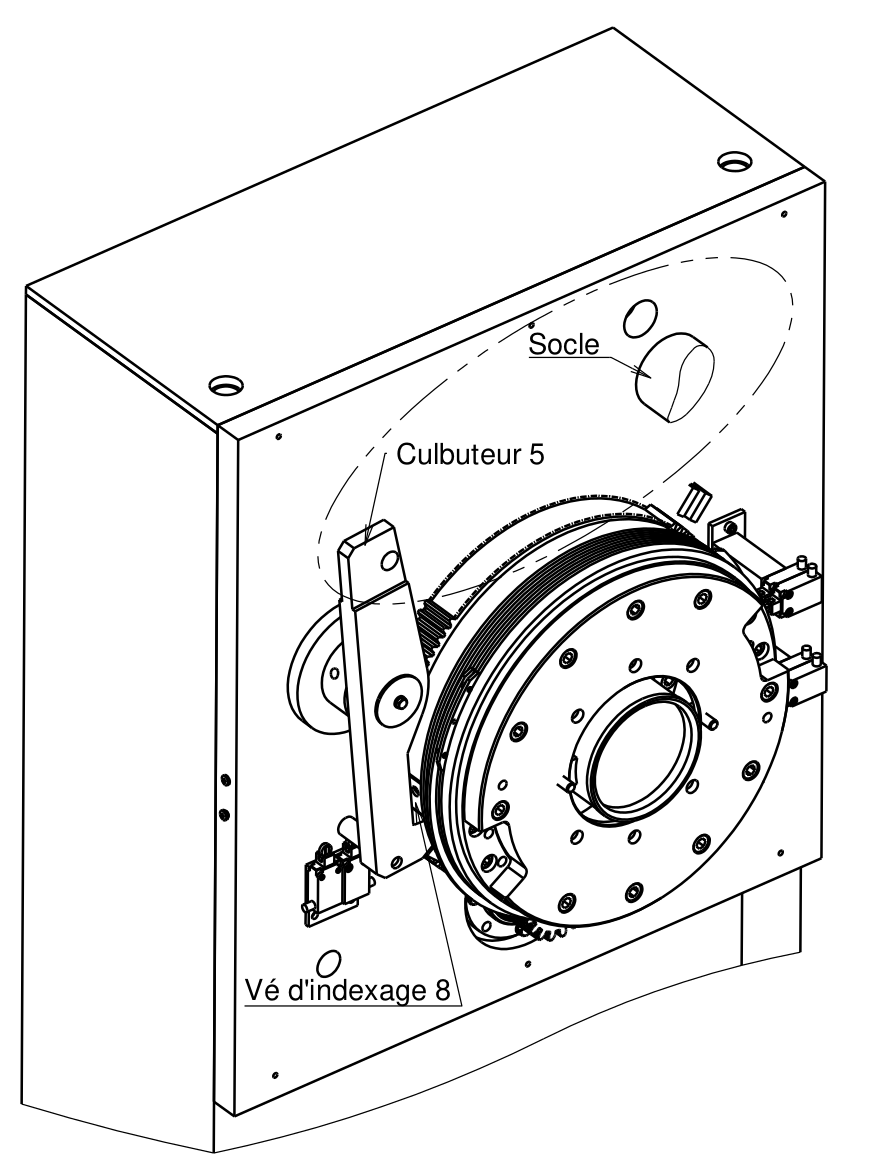
\includegraphics[width=0.95\linewidth]{img/fig10}
 \caption{Emplacement du vé d’indexage 8 et du vérin électrique à implanter}
 \label{img10}
\end{minipage}
\end{figure}

\subsection{Montage d’un galet 8’ sur le vé d’indexage 8}

\begin{figure}[!h]
\centering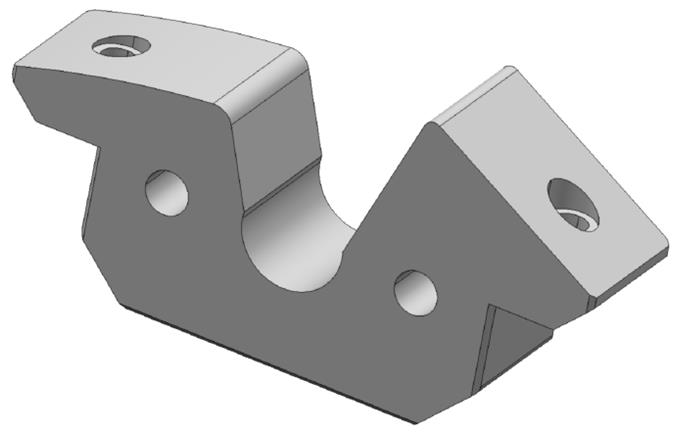
\includegraphics[width=0.6\linewidth]{img/fig11}
 \caption{Vé d’indexage 8 (pièce avant modification)}
 \label{img11}
\end{figure}

\begin{figure}[!h]
\centering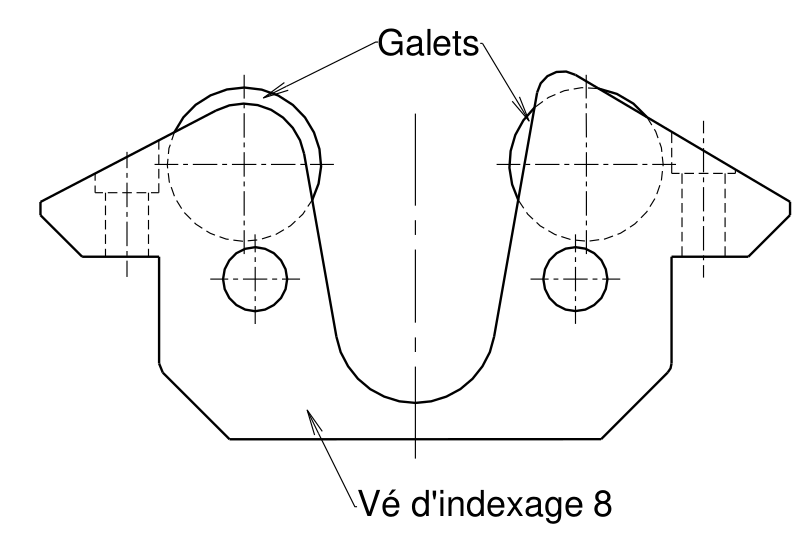
\includegraphics[width=0.6\linewidth]{img/fig12}
 \caption{Positionnement des galets sur le vé d’indexage 8}
 \label{img12}
\end{figure}

\question{En vous inspirant du formalisme des schémas technologiques des figures \ref{img14} et \ref{img15}, sur le document réponse, réaliser un schéma technologique de votre proposition de solution pour le montage d’un galet 8’ sur un vé d’indexage 8.}

\paragraph{Présentation du support de travail graphique :}

Pour cette partie de l’étude, il vous est demandé de définir plusieurs sous-ensembles du mécanisme sur le calque format A3 fourni avec le sujet. Les éléments pré-imprimés sur ce calque sont destinés à faciliter la mise en place des différents composants.

\begin{figure}[!h]
\centering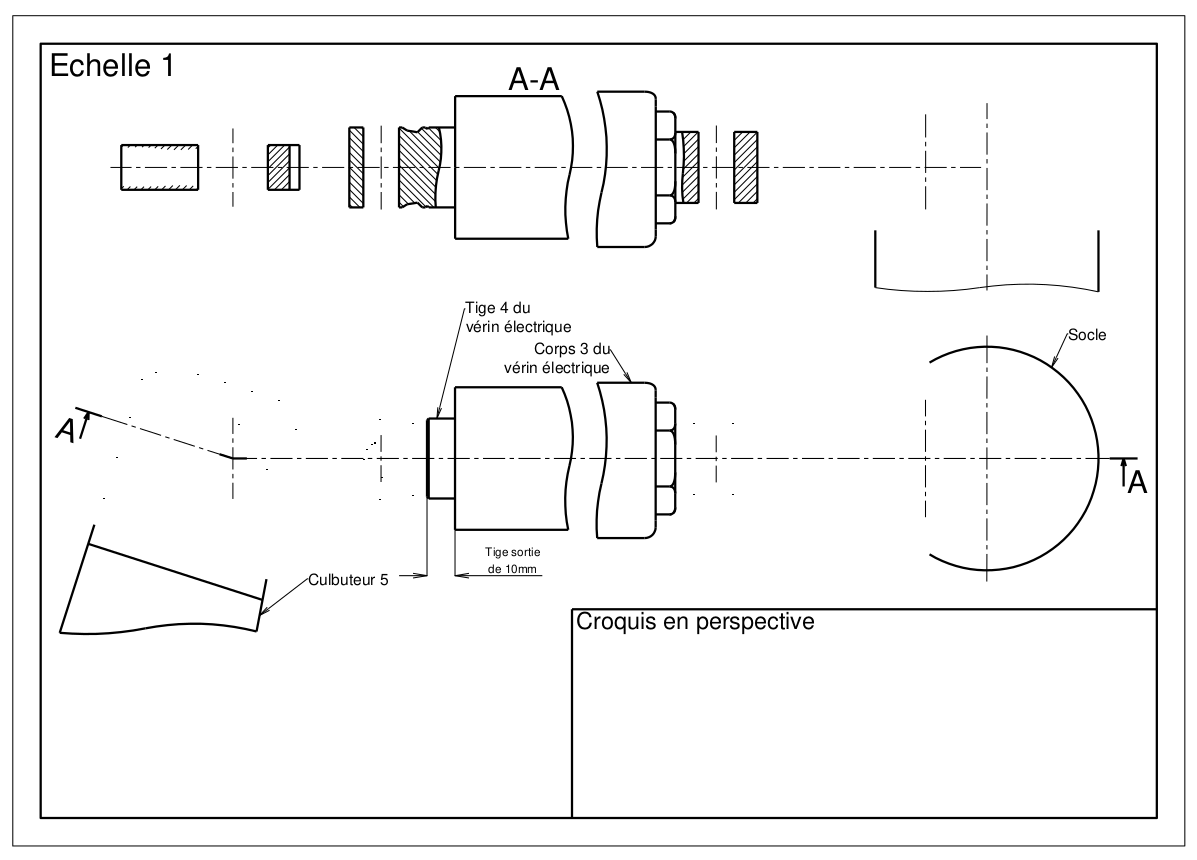
\includegraphics[width=0.6\linewidth]{img/fig13}
 \caption{Mise en page du calque à compléter}
 \label{img13}
\end{figure}

Pour des raisons d’encombrement, les vues sont interrompues, seules les extrémités du vérin électrique sont représentées afin de relier celui-ci au système existant.

\paragraph{Consignes spécifiques aux travaux graphiques}

Les candidats doivent fournir des dessins traduisant sans ambiguïté leurs intentions de conception. Pour cela, les candidats sont invités à faire preuve de rigueur dans leur tracé (en particulier, l’utilisation d’une règle ne pourra être que conseillée) et à donner toutes les
précisions qu’ils jugeront pertinentes afin de permettre au correcteur d’évaluer la qualité de leurs solutions.

Les principales conditions fonctionnelles relatives aux liaisons représentées seront clairement indiquées en respectant les règles normalisées AFNOR.

Les éléments normalisés utilisés par le candidat autres que ceux fournis dans le sujet, seront dessinés approximativement en respectant au mieux leurs proportions.

Toute vue complémentaire est laissée à l’initiative du candidat.

\paragraph{Liaison Tige de vérin 4-Culbuteur 5}

L’objectif est de réaliser une liaison pivot entre la tige du vérin électrique 4 et le culbuteur 5.

Pour cela une pièce intermédiaire appelée chape a été partiellement  mise en place sur le dessin.

\paragraph{Données :}
\begin{itemize}
 \item Les formes du culbuteur existant sont conservées. Des usinages supplémentaires peuvent être ajoutés (perçage, taraudage, lamage...).
 \item La chape doit être en liaison encastrement démontable avec l’extrémité de la tige du vérin électrique.
 \item La liaison entre la chape et le culbuteur 5 est une liaison pivot réalisée à l’aide de deux paliers iglidur® J de référence JFM-2528-06 (voir annexe F).
 \item En position déverrouillée la tige du vérin est sortie d’environ 10mm. La tige du vérin doit pouvoir rentrer totalement.
 \item Aucun usinage supplémentaire n’est possible sur la tige du vérin.
\end{itemize}

Schéma de la solution technologique retenue :

\begin{figure}[!h]
\centering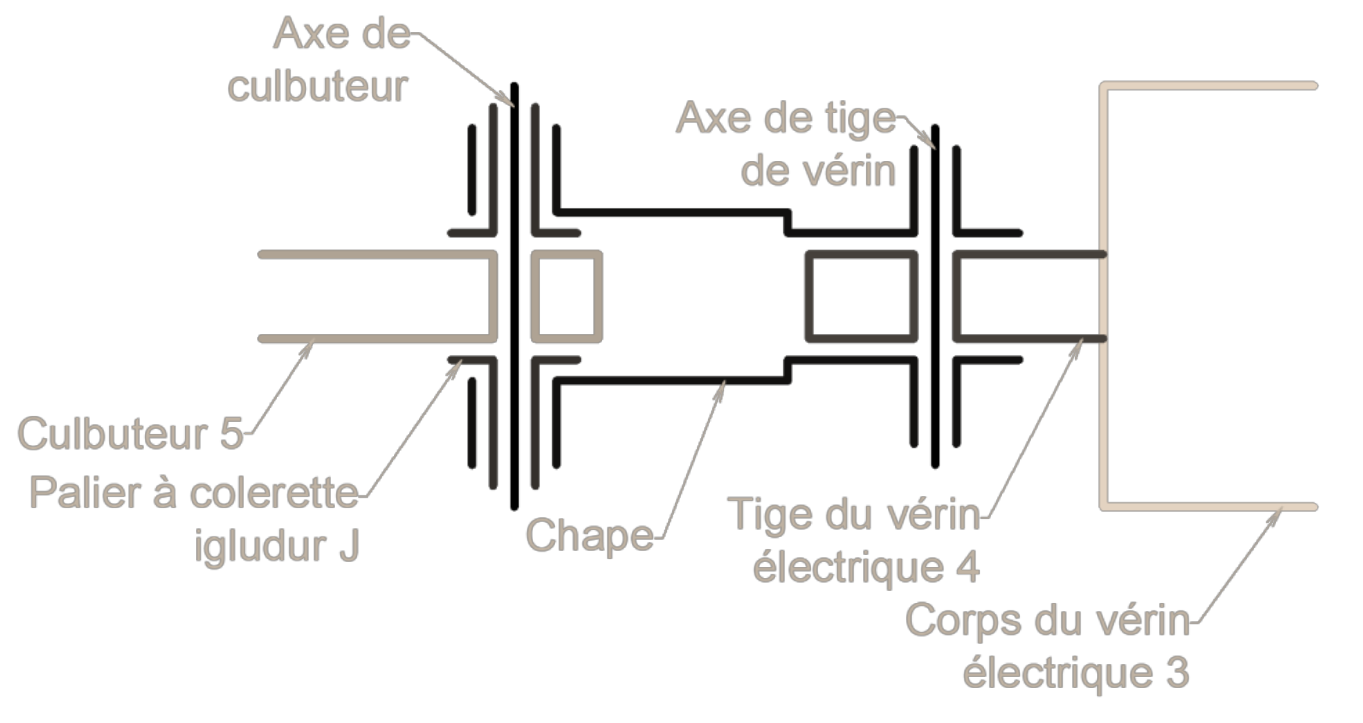
\includegraphics[width=0.6\linewidth]{img/fig14}
 \caption{Schéma de la solution technologique retenue pour la liaison vérin 4 / culbuteur 5}
 \label{img14}
\end{figure}

\question{Définir graphiquement votre proposition de solution en vue extérieure et en vue en coupe A-A (à l’échelle 1).

Sur la vue en coupe A-A, seules les arrêtes cachées permettant de
montrer la possibilité du débattement angulaire seront représentées.

Les ajustements (normalisés ou non) sont à préciser.

Les arrêts en translation des axes de tige de vérin et de culbuteur doivent être définis.}

\newpage

\subsection{Liaison Corps de vérin 3 – Socle}

L’objectif est de réaliser une liaison linéaire annulaire entre le corps du vérin électrique 3 et le socle. Pour cela une pièce intermédiaire appelée noix  a été partiellement  mise en place sur le dessin.

\paragraph{Données :}
\begin{itemize}
 \item Le socle de fixation du corps du vérin reste identique au niveau des formes extérieures (Cylindre de révolution de diamètre 80mm). Sa partie supérieure permettant de réaliser la liaison linéaire annulaire entre le corps du vérin et le socle sera entièrement redéfinie,
 \item L’axe de la liaison linéaire annulaire est coplanaire à l’axe de la liaison pivot entre le vérin électrique et le culbuteur,
 \item La noix doit être en liaison complète démontable avec l’extrémité du corps vérin électrique,
 \item Aucun usinage supplémentaire n’est possible sur le corps du vérin,
 \item La noix sera liée au socle par l’intermédiaire d’une liaison rotule standard (voir annexe G),
 \item La liaison noix / rotule sera une liaison complète réglable axialement,
 \item La liaison rotule / socle sera une liaison pivot glissant avec un débattement axial de 1mm mini de chaque côté,
 \item Pour réaliser la liaison pivot glissant, une vis axe peut être utilisée (voir annexe G).
\end{itemize}

Schéma de la solution technologique retenue :

\begin{figure}[!h]
\centering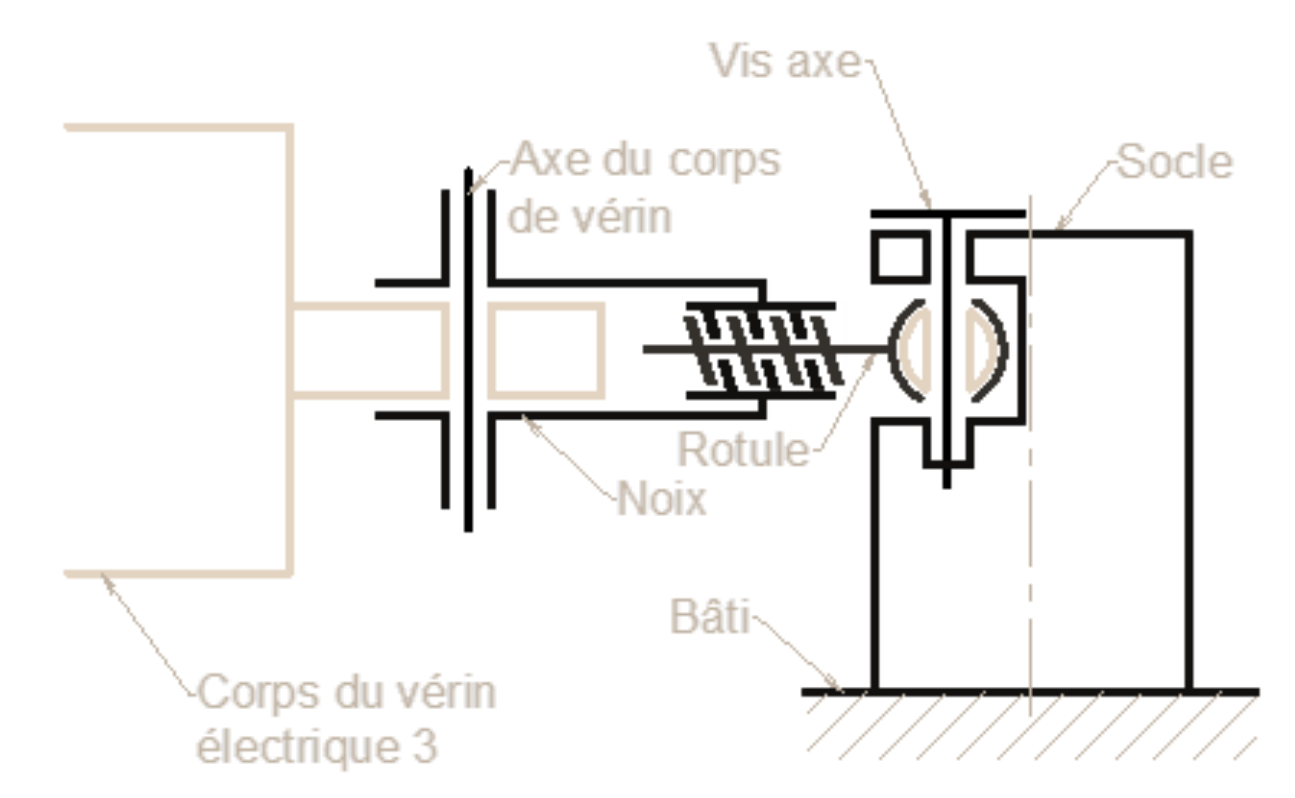
\includegraphics[width=0.6\linewidth]{img/fig15}
 \caption{Schéma de la solution technologique retenue pour la liaison corps de vérin 3/socle}
 \label{img15}
\end{figure}

\question{Définir graphiquement votre proposition de solution en vue extérieure et en vue en coupe A-A. Sur la vue en coupe A-A, seules les arrêtes cachées permettant de montrer la possibilité du débattement angulaire seront représentées.

Les ajustements (normalisés ou non) sont à préciser.

Les arrêts en translation de l’axe du corps du vérin doivent être définis.}

~\

\begin{center}
\Large{--- Fin du sujet ---}
\end{center}

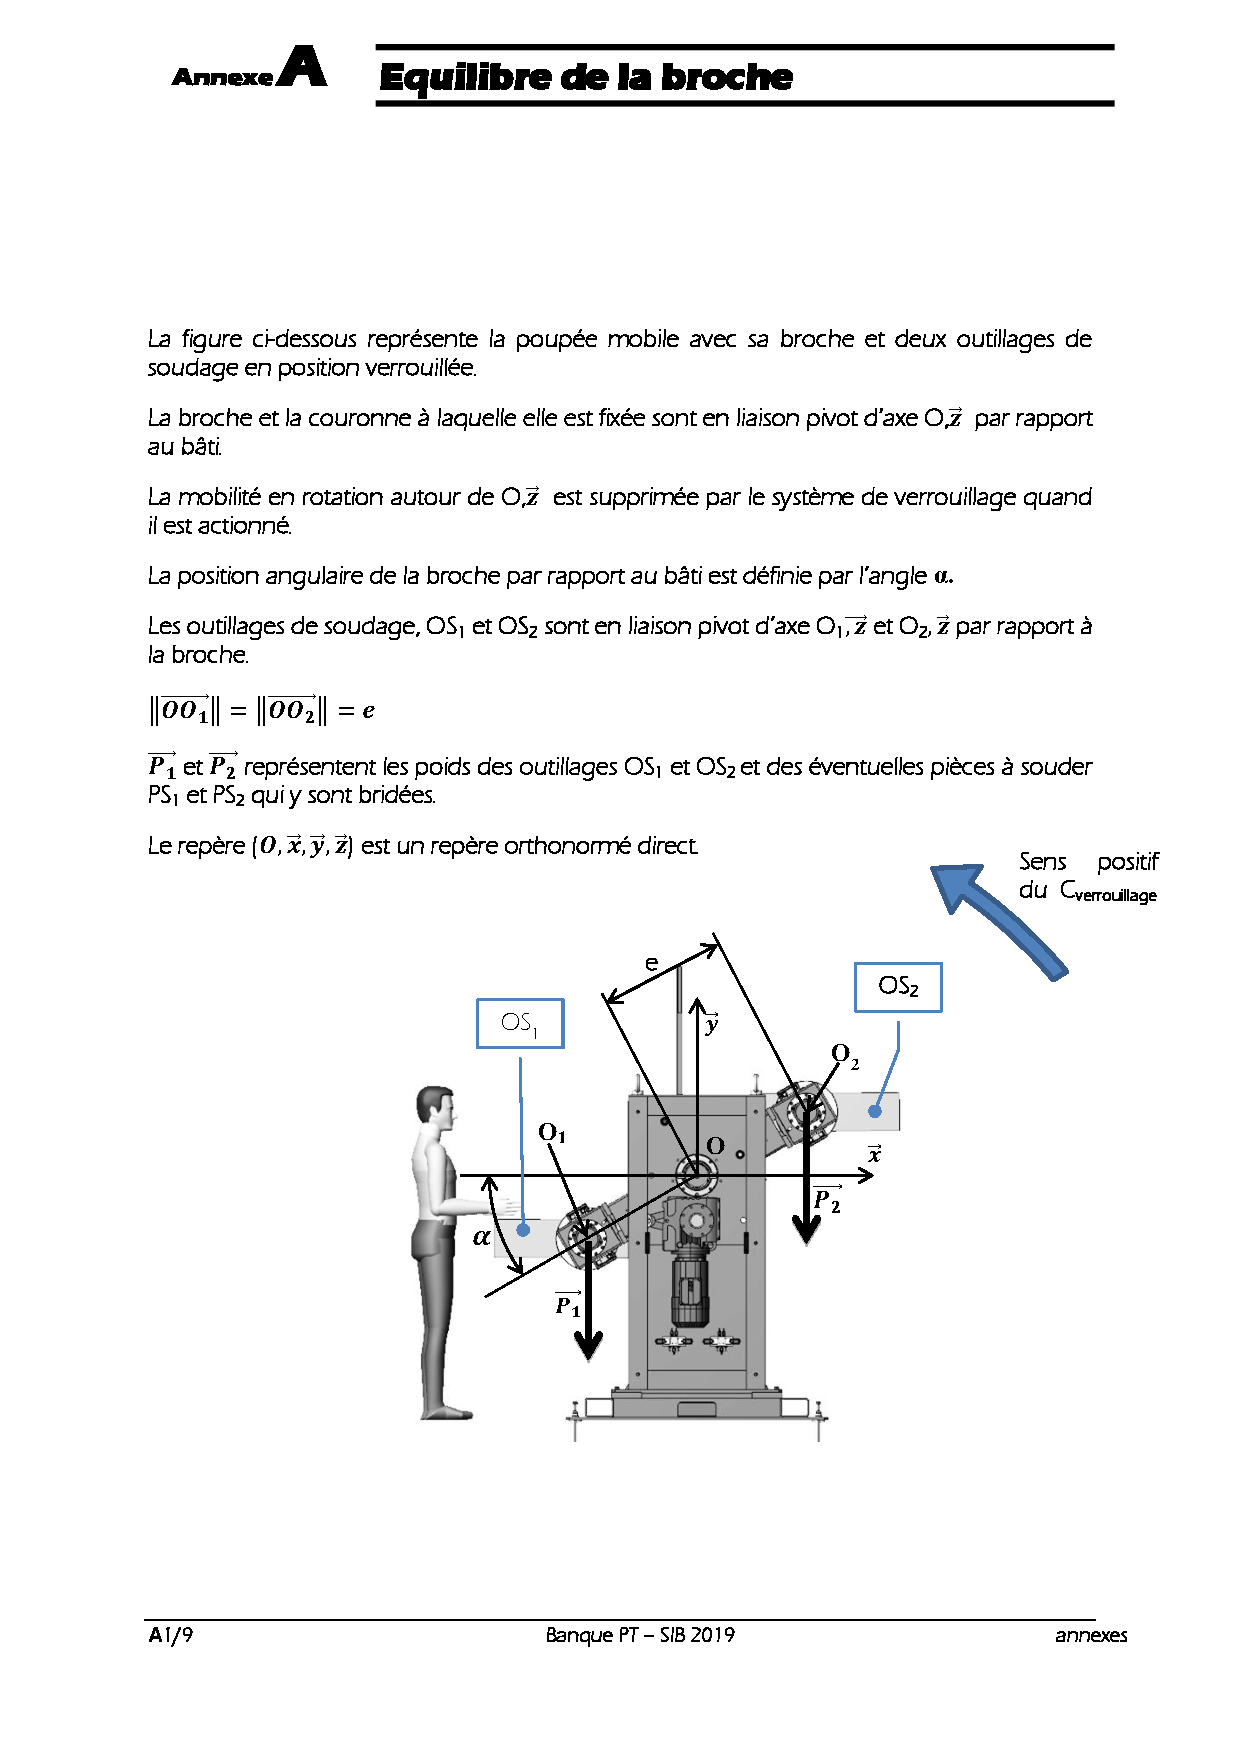
\includepdf[offset=0mm -10mm,pages=-]{img/annexes}

\cleardoublepage

\ifdef{\public}{\pagestyle{documentreponse}}{\pagestyle{correction}}

\reponse{0}{\begin{center}
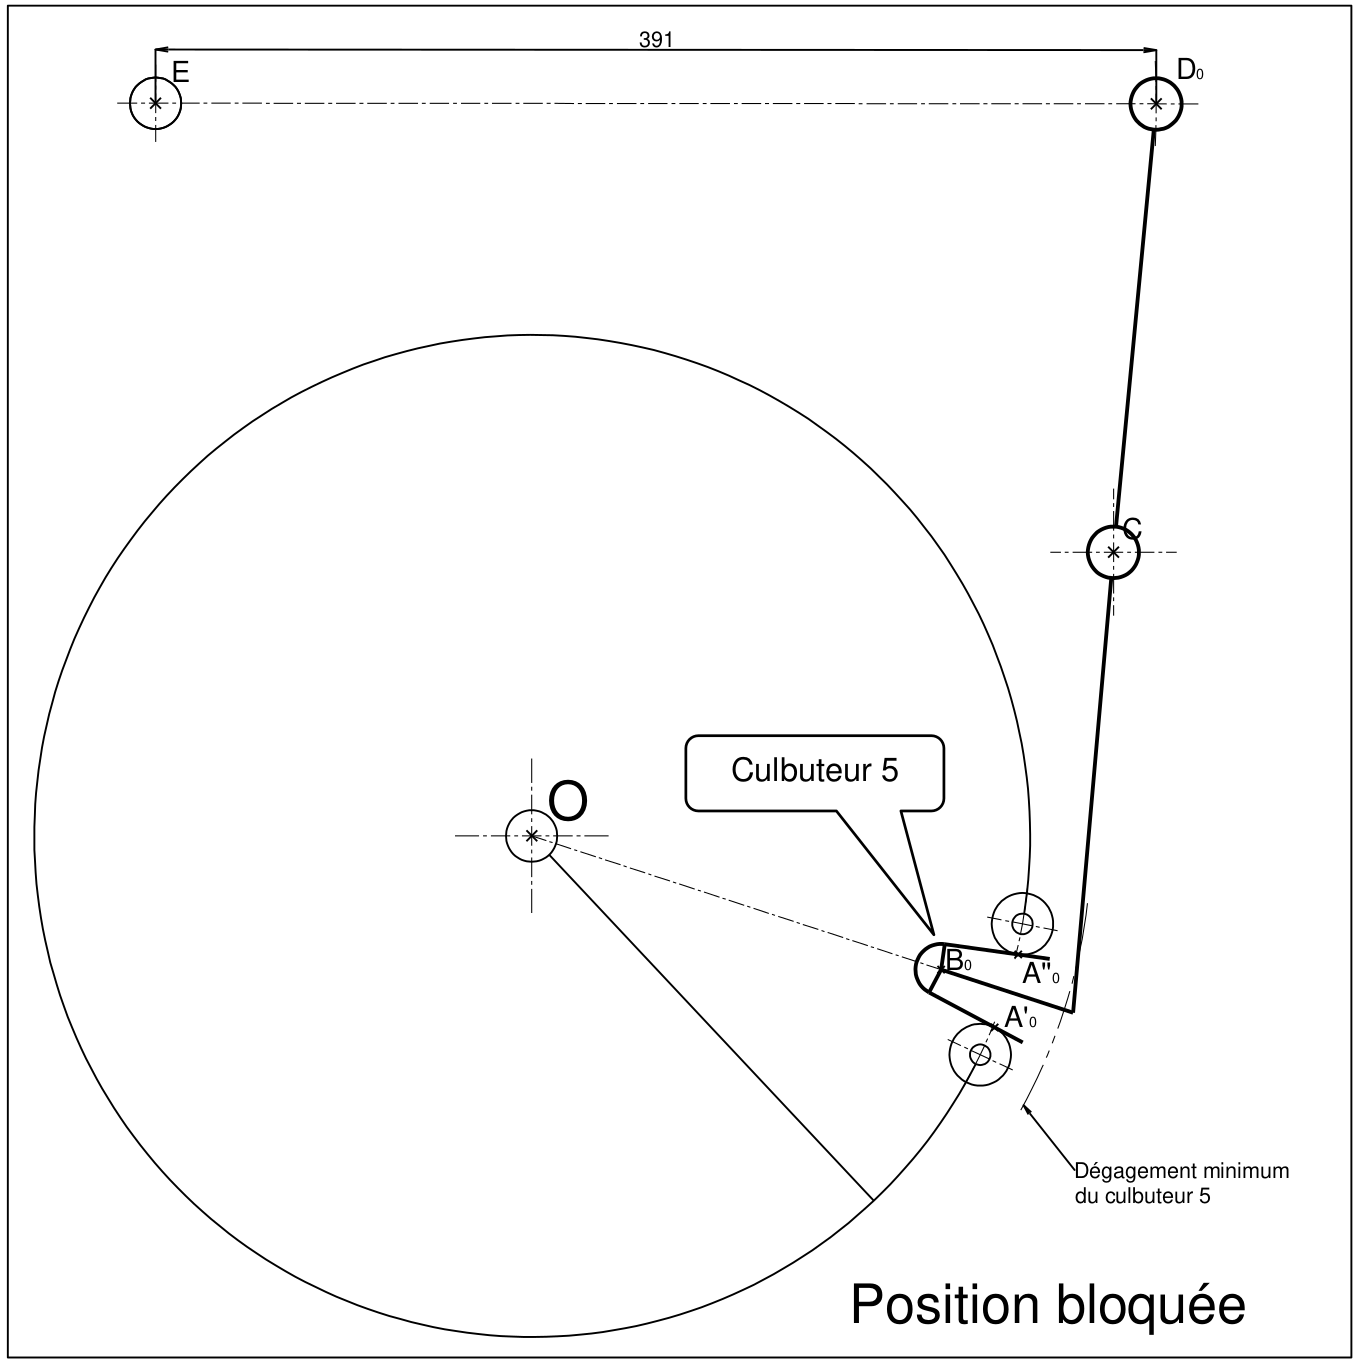
\includegraphics[width=0.9\linewidth]{img/DR01}
\end{center}\vspace{-1cm}}{
\begin{center}
\begin{tikzpicture}

% Include the image in a node
\node [above right,inner sep=0] (image) at (0,0) {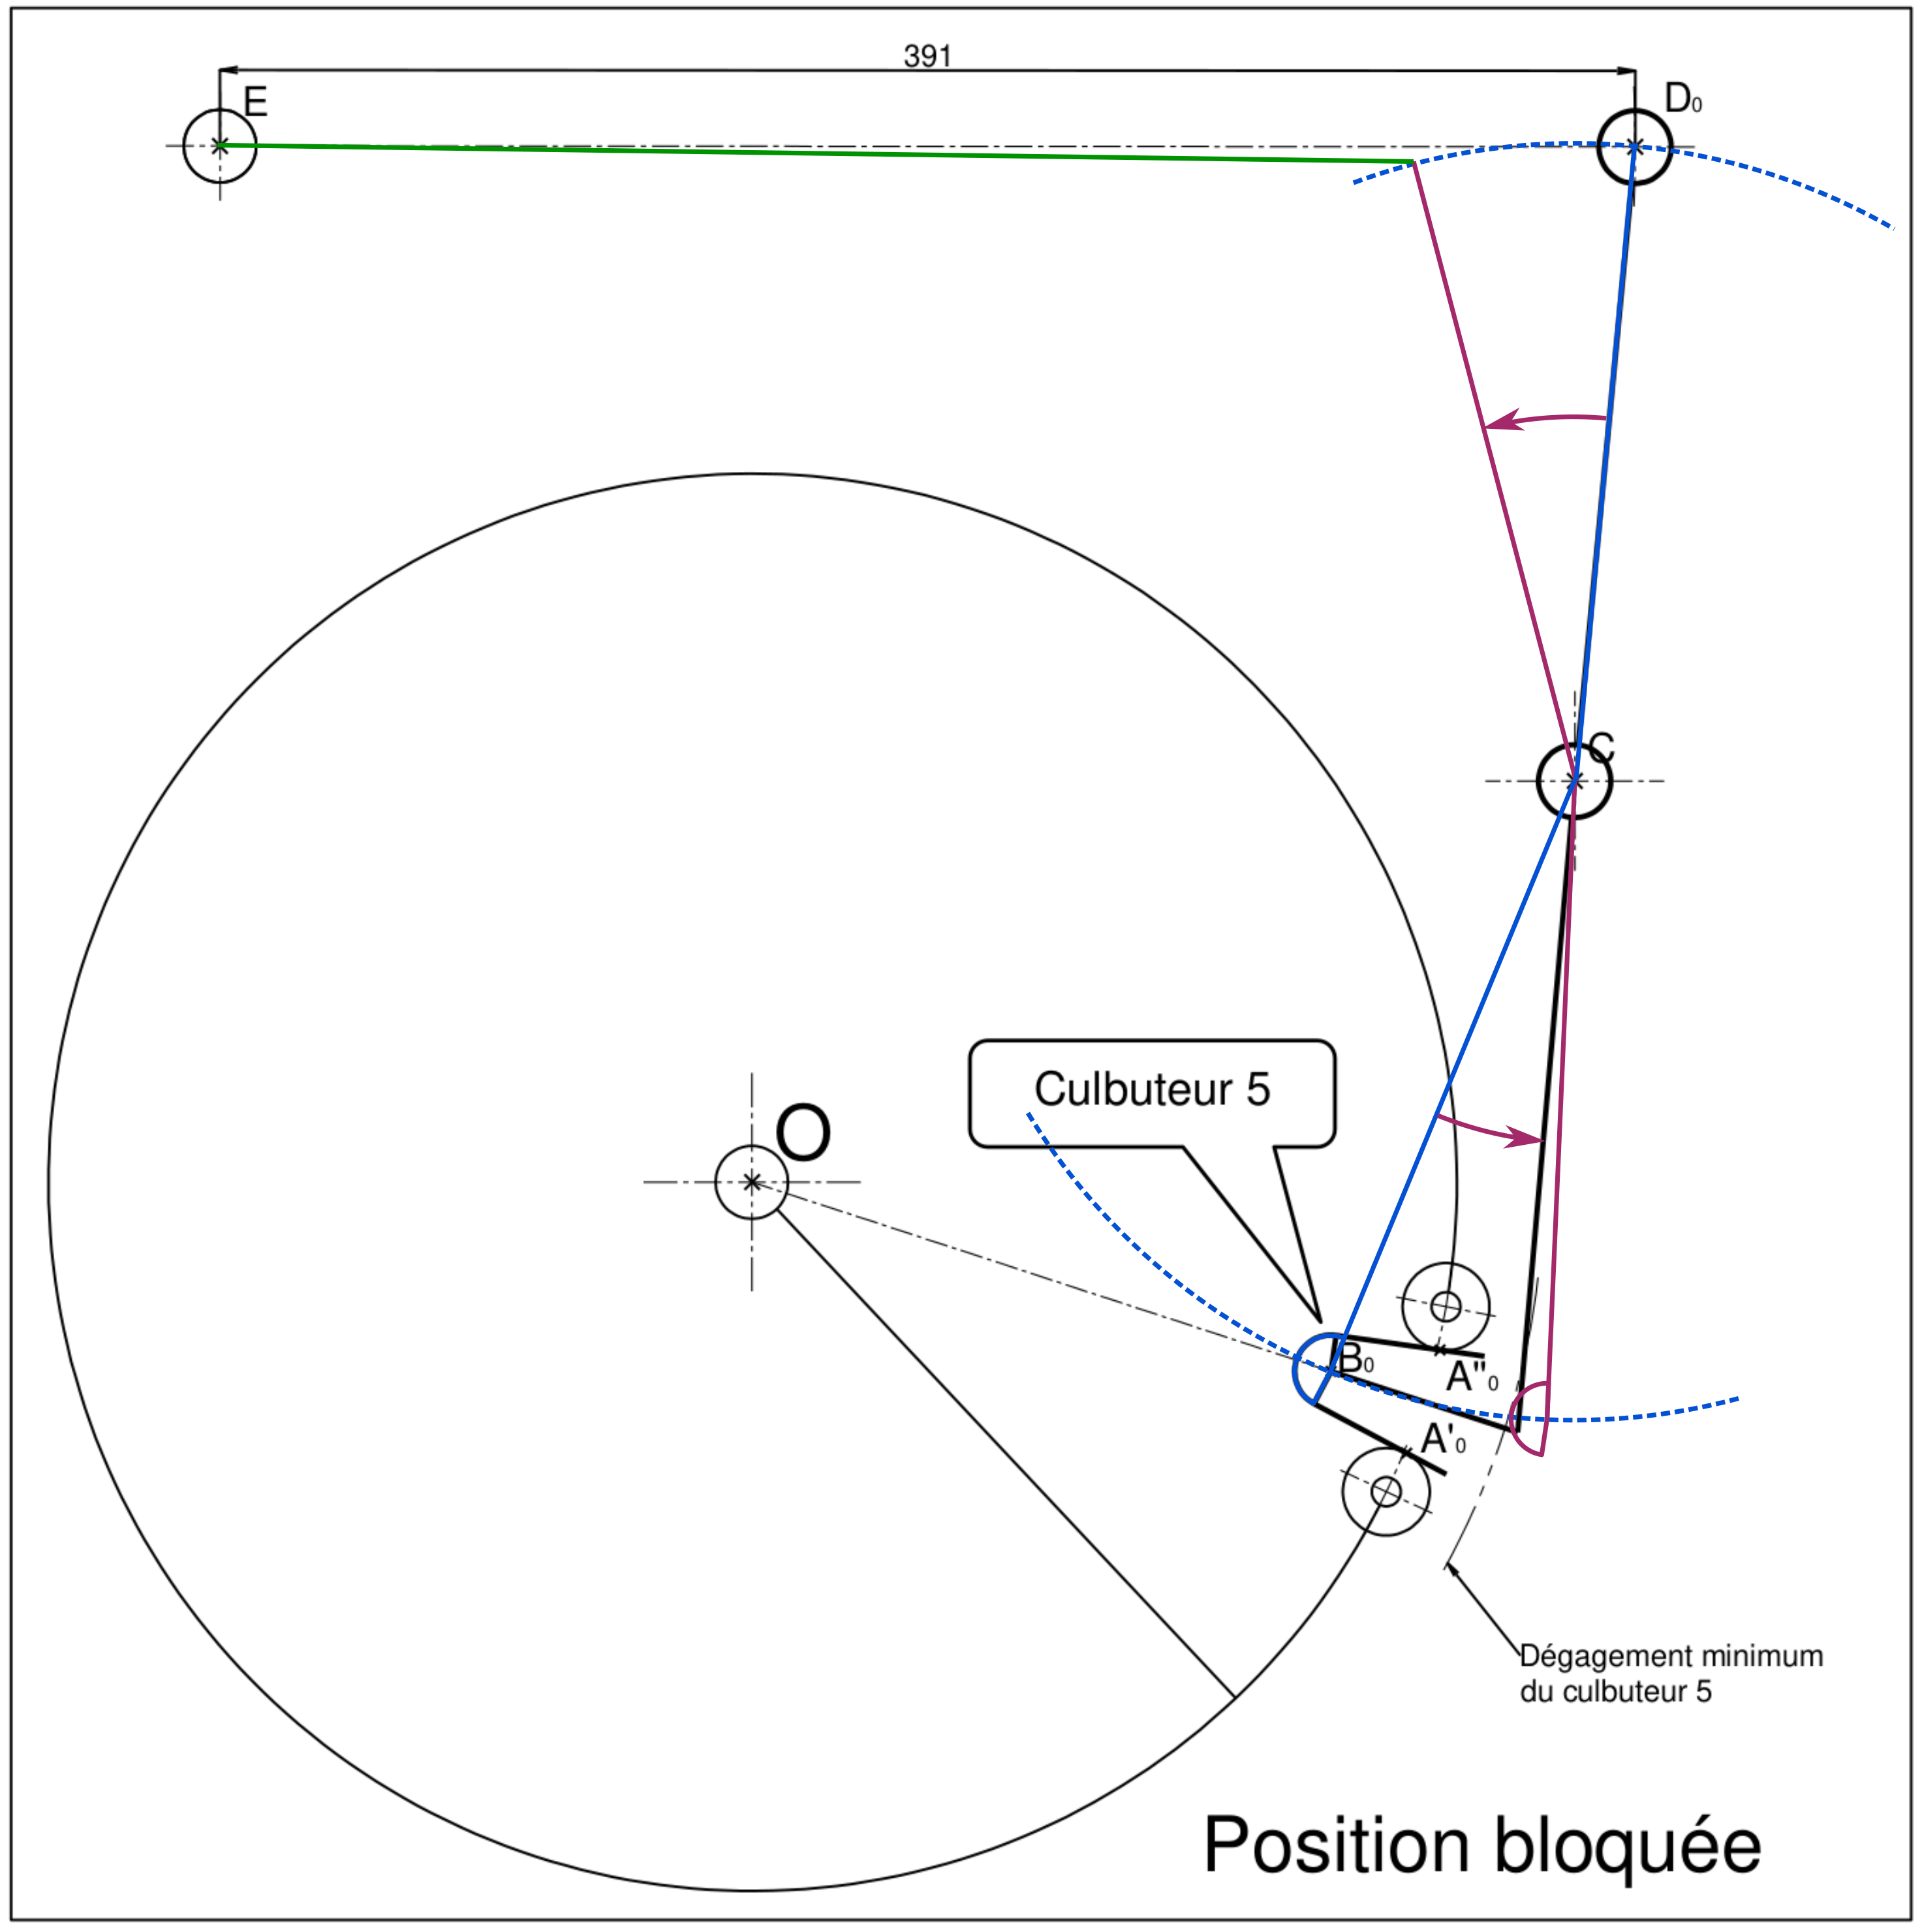
\includegraphics[width=0.9\linewidth]{img/DR01_cor}};
%	\draw[lightgray,step=1] (image.south west) grid (image.north east);
	\node at (12.6,4.3){$B_1$};
	\node at (11.8,6.6){$\alpha$};
	\node at (12.3,12.3){$\alpha$};
	\node at (11,13.6){$D_1$};
	\node at (6.8,13.7){325};
\end{tikzpicture}
\end{center}
}

\reponse{5}{}{\begin{itemize}
 \item $L_{max}=391mm$,
 \item $L_{min}=325mm$ (mesuré sur la figure précédente),
 \item $C_{min}=66mm$ 
\end{itemize}
}

\reponse{5}{}{$C_{verrouillage}=\left(\overrightarrow{OO_1}\wedge\vec{P}_1+\overrightarrow{OO_2}\wedge\vec{P}_2\right)\cdot\vec{z}=e\cdot cos\alpha\cdot \left(\vec{P}_1-\vec{P}_2\right)$
}

\reponse{0}{\begin{center}
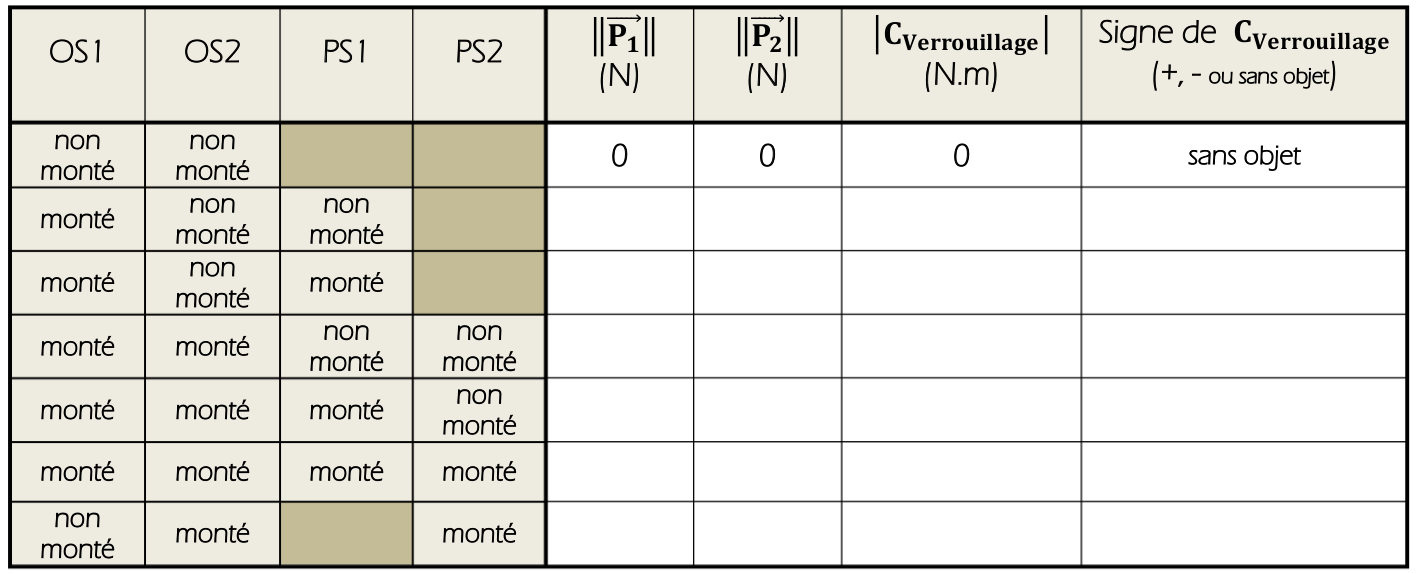
\includegraphics[width=0.9\linewidth]{img/DR02}
\end{center}\vspace{-1cm}}{
\begin{center}
\begin{tikzpicture}

% Include the image in a node
\node [above right,inner sep=0] (image) at (0,0) {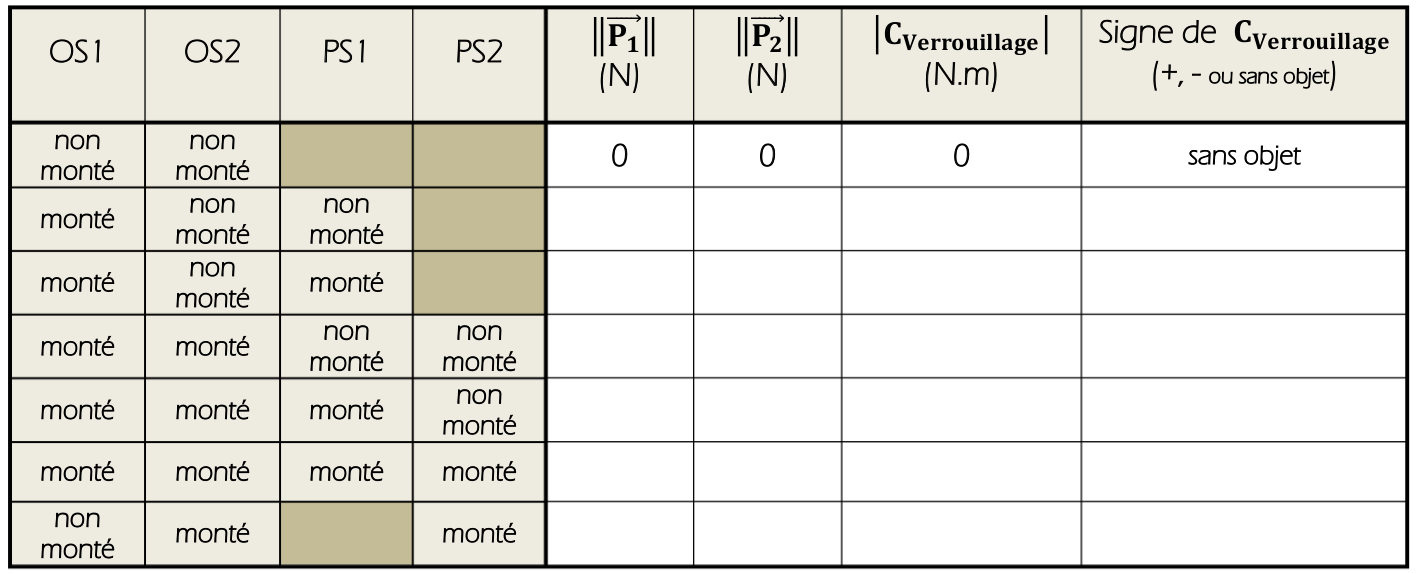
\includegraphics[width=0.9\linewidth]{img/DR02}};
%	\draw[lightgray,step=1] (image.south west) grid (image.north east);
	\node at (6.7,0.4){$0$};
	\node at (8.2,0.4){$3000$};
	\node at (6.7,1.1){$3000$};
	\node at (8.2,1.1){$3000$};
	\node at (6.7,1.8){$3000$};
	\node at (8.2,1.8){$1000$};
	\node at (6.7,2.4){$1000$};
	\node at (8.2,2.4){$1000$};
	\node at (6.7,3.1){$3000$};
	\node at (8.2,3.1){$0$};
	\node at (6.7,3.8){$1000$};
	\node at (8.2,3.8){$0$};
	\node at (10.2,0.4){$1,96.10^3$};
	\node at (13.3,0.4){-};
	\node at (10.2,1.1){$0$};
	\node at (13.3,1.1){sans objet};
	\node at (10.2,1.8){$1,31.10^3$};
	\node at (13.3,1.8){+};
	\node at (10.2,2.4){$0$};
	\node at (13.3,2.4){sans objet};
	\node at (10.2,3.1){$1,96.10^3$};
	\node at (13.3,3.1){+};
	\node at (10.2,3.8){$653$};
	\node at (13.3,3.8){+};
\end{tikzpicture}
\end{center}
}

\reponse{5}{}{\begin{itemize}
 \item Sens positif: $\left|C_{verouillage}\right|_{max}=1.96\cdot10^3N.m$,
 \item Sens négatif: $\left|C_{verouillage}\right|_{max}=1.96\cdot10^3N.m$. 
\end{itemize}
}

\ifdef{\public}{\newpage}

\reponse{3}{}{Il est le plus utilisé en phase de réglage car c'est dans ce cas là qu'il n'y a qu'un seul outillage et une seule pièce.
}

\reponse{3}{}{Il s'agit du Théorème du Moment Statique appliqué en O et projeté sur $\vec{z}$.}


\reponse{0}{\begin{center}
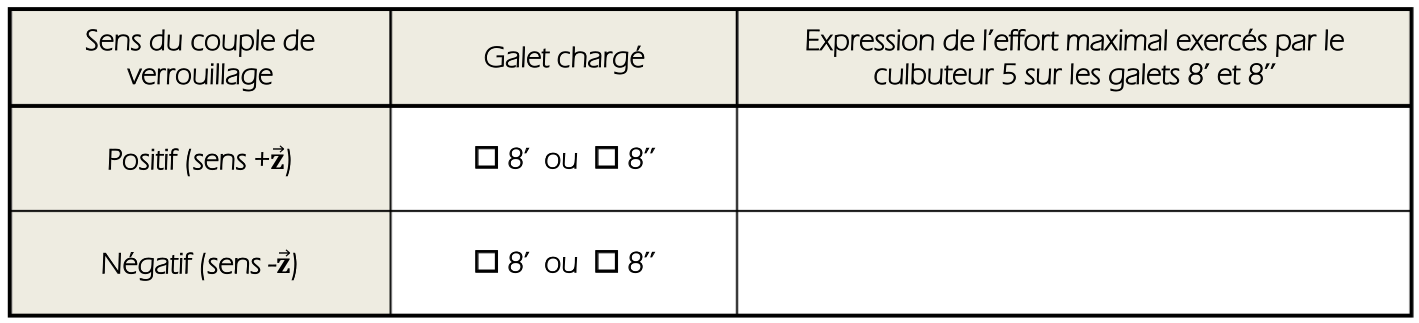
\includegraphics[width=0.8\linewidth]{img/DR03}
\end{center}\vspace{-1cm}}{
\begin{center}
\begin{tikzpicture}

% Include the image in a node
\node [above right,inner sep=0] (image) at (0,0) {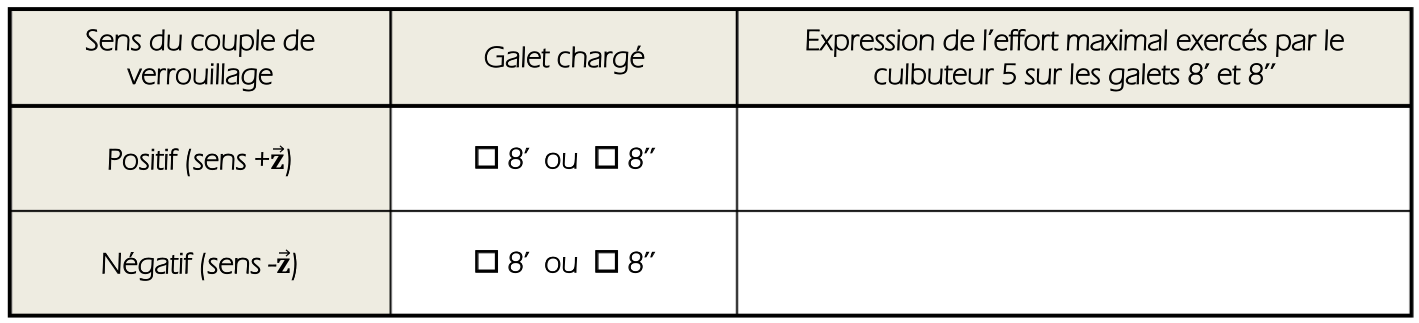
\includegraphics[width=0.9\linewidth]{img/DR03}};
%	\draw[lightgray,step=1] (image.south west) grid (image.north east);
    \node at (6.5,0.65){x};
    \node at (5.2,1.8){x};
	\node at (11.2,1.8){$\left\|\overrightarrow{A'_{5/8'}}\right\|=\frac{\left|C_{verrouillage}\right|_{max}}{r\cdot cos \beta}$};
	\node at (11.2,0.6){$\left\|\overrightarrow{A''_{5/8''}}\right\|=\frac{\left|C_{verrouillage}\right|_{max}}{r\cdot cos \beta}$};
\end{tikzpicture}
\end{center}

P.F.S. en O et en projection sue $\vec{z}$: $\left|C_{verrouillage}\right|_{max}+\left(\overrightarrow{OA'_0}\wedge \left\|\overrightarrow{A'_{5/8'}}\right\|_{max}\cdot \vec{y}'_{02}\right)\cdot\vec{z}=0$, donc $\left|C_{verrouillage}\right|_{max}=r\cdot\left\|\overrightarrow{A'_{5/8'}}\right\|_{max}\cdot cos \beta$.

Il en va de même pour le couple négatif.
}

\reponse{5}{}{
$Fr_{B_max}=\left\|\overrightarrow{A'_{5/8'}}\right\|_{max}=\left\|\overrightarrow{A''_{5/8''}}\right\|_{max}=\frac{\left|C_{verrouillage}\right|_{max}}{r\cdot cos \beta}=\frac{2000}{0,2\cdot cos\beta}$

Comme $2\cdot\beta+2\cdot\delta=20\degree$, donc $\beta+\delta=10\degree$ et $\beta<10\degree$, on retient ainsi $cos\beta\approx0,99$

$Fr_{B_max}\approx \frac{2000}{0,2\cdot 0.99}\approx 10,1\cdot 10^3N$
}

\ifdef{\public}{\newpage}


\reponse{5}{}{
Désignation: NATV8PPA
}


\reponse{13}{\begin{itemize}
 \item $\overrightarrow{A'_{+18'/5}}=\left\{\begin{array}{l}
 Point\ d'application:\ A'_{+1}\\
 Direction:\ perpendiculaire\ au\ culbuteur\\
 Norme:\ connue
 \end{array}
 \right.$
 \end{itemize}
}{
Le culbuteur est soumis à 3 actions mécaniques:
\begin{itemize}
 \item $\overrightarrow{A'_{+18'/5}}\left\{\begin{array}{l}
 Point\ d'application:\ A'_{+1}\\
 Direction:\ perpendiculaire\ au\ culbuteur\\
 Norme:\ connue
 \end{array}
 \right.$
 \item $\overrightarrow{D_{+14/5}}\left\{\begin{array}{l}
 Point\ d'application:\ D_{+1}\\
 Direction:\ axe\ de\ la \ tige\ 4\\
 Norme:\ inconnue
 \end{array}
 \right.$
 \item $\overrightarrow{C_{+1bati/5}}\left\{\begin{array}{l}
 Point\ d'application:\ C\\
 Direction:\ inconnue\\
 Norme:\ inconnue
 \end{array}
 \right.$ 
\end{itemize}
}

\reponse{0}{\begin{center}
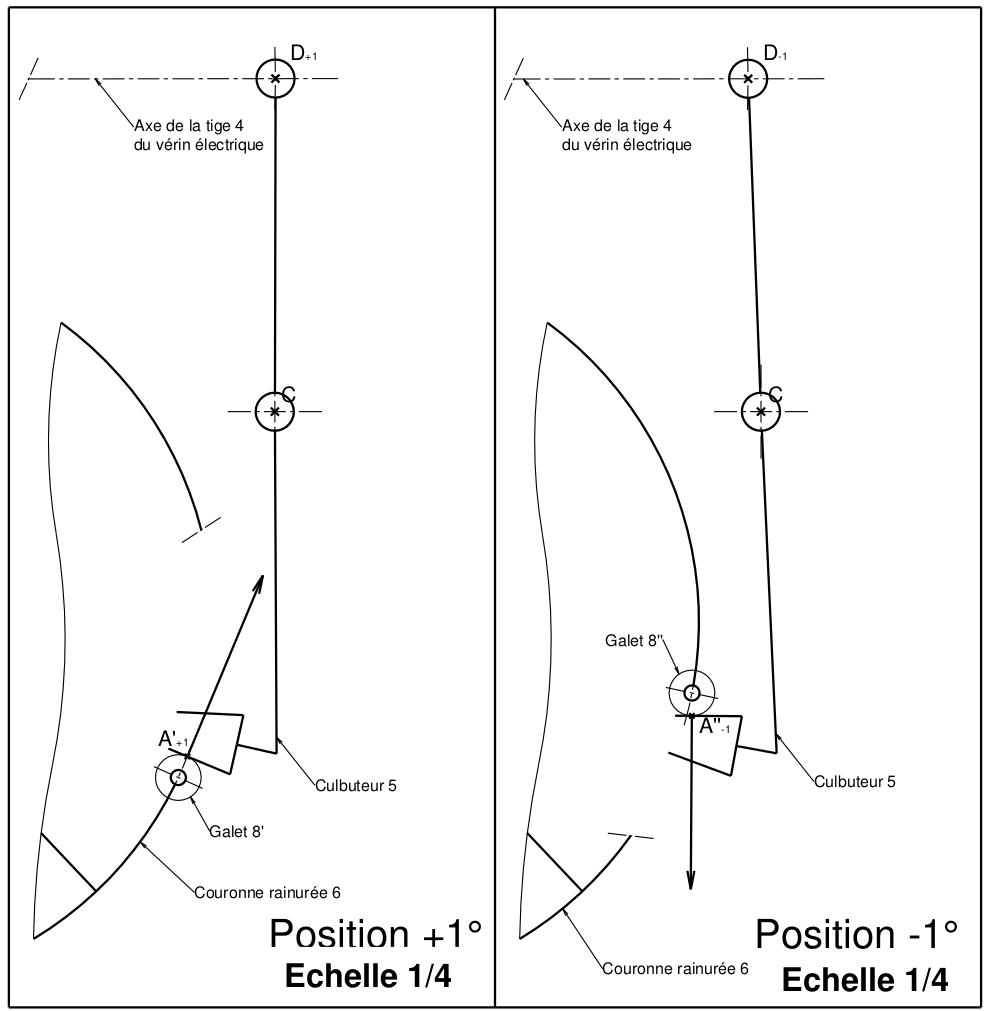
\includegraphics[width=0.9\linewidth]{img/DR04}
\end{center}\vspace{-1cm}}{
\begin{center}
\begin{tikzpicture}

% Include the image in a node
\node [above right,inner sep=0] (image) at (0,0) {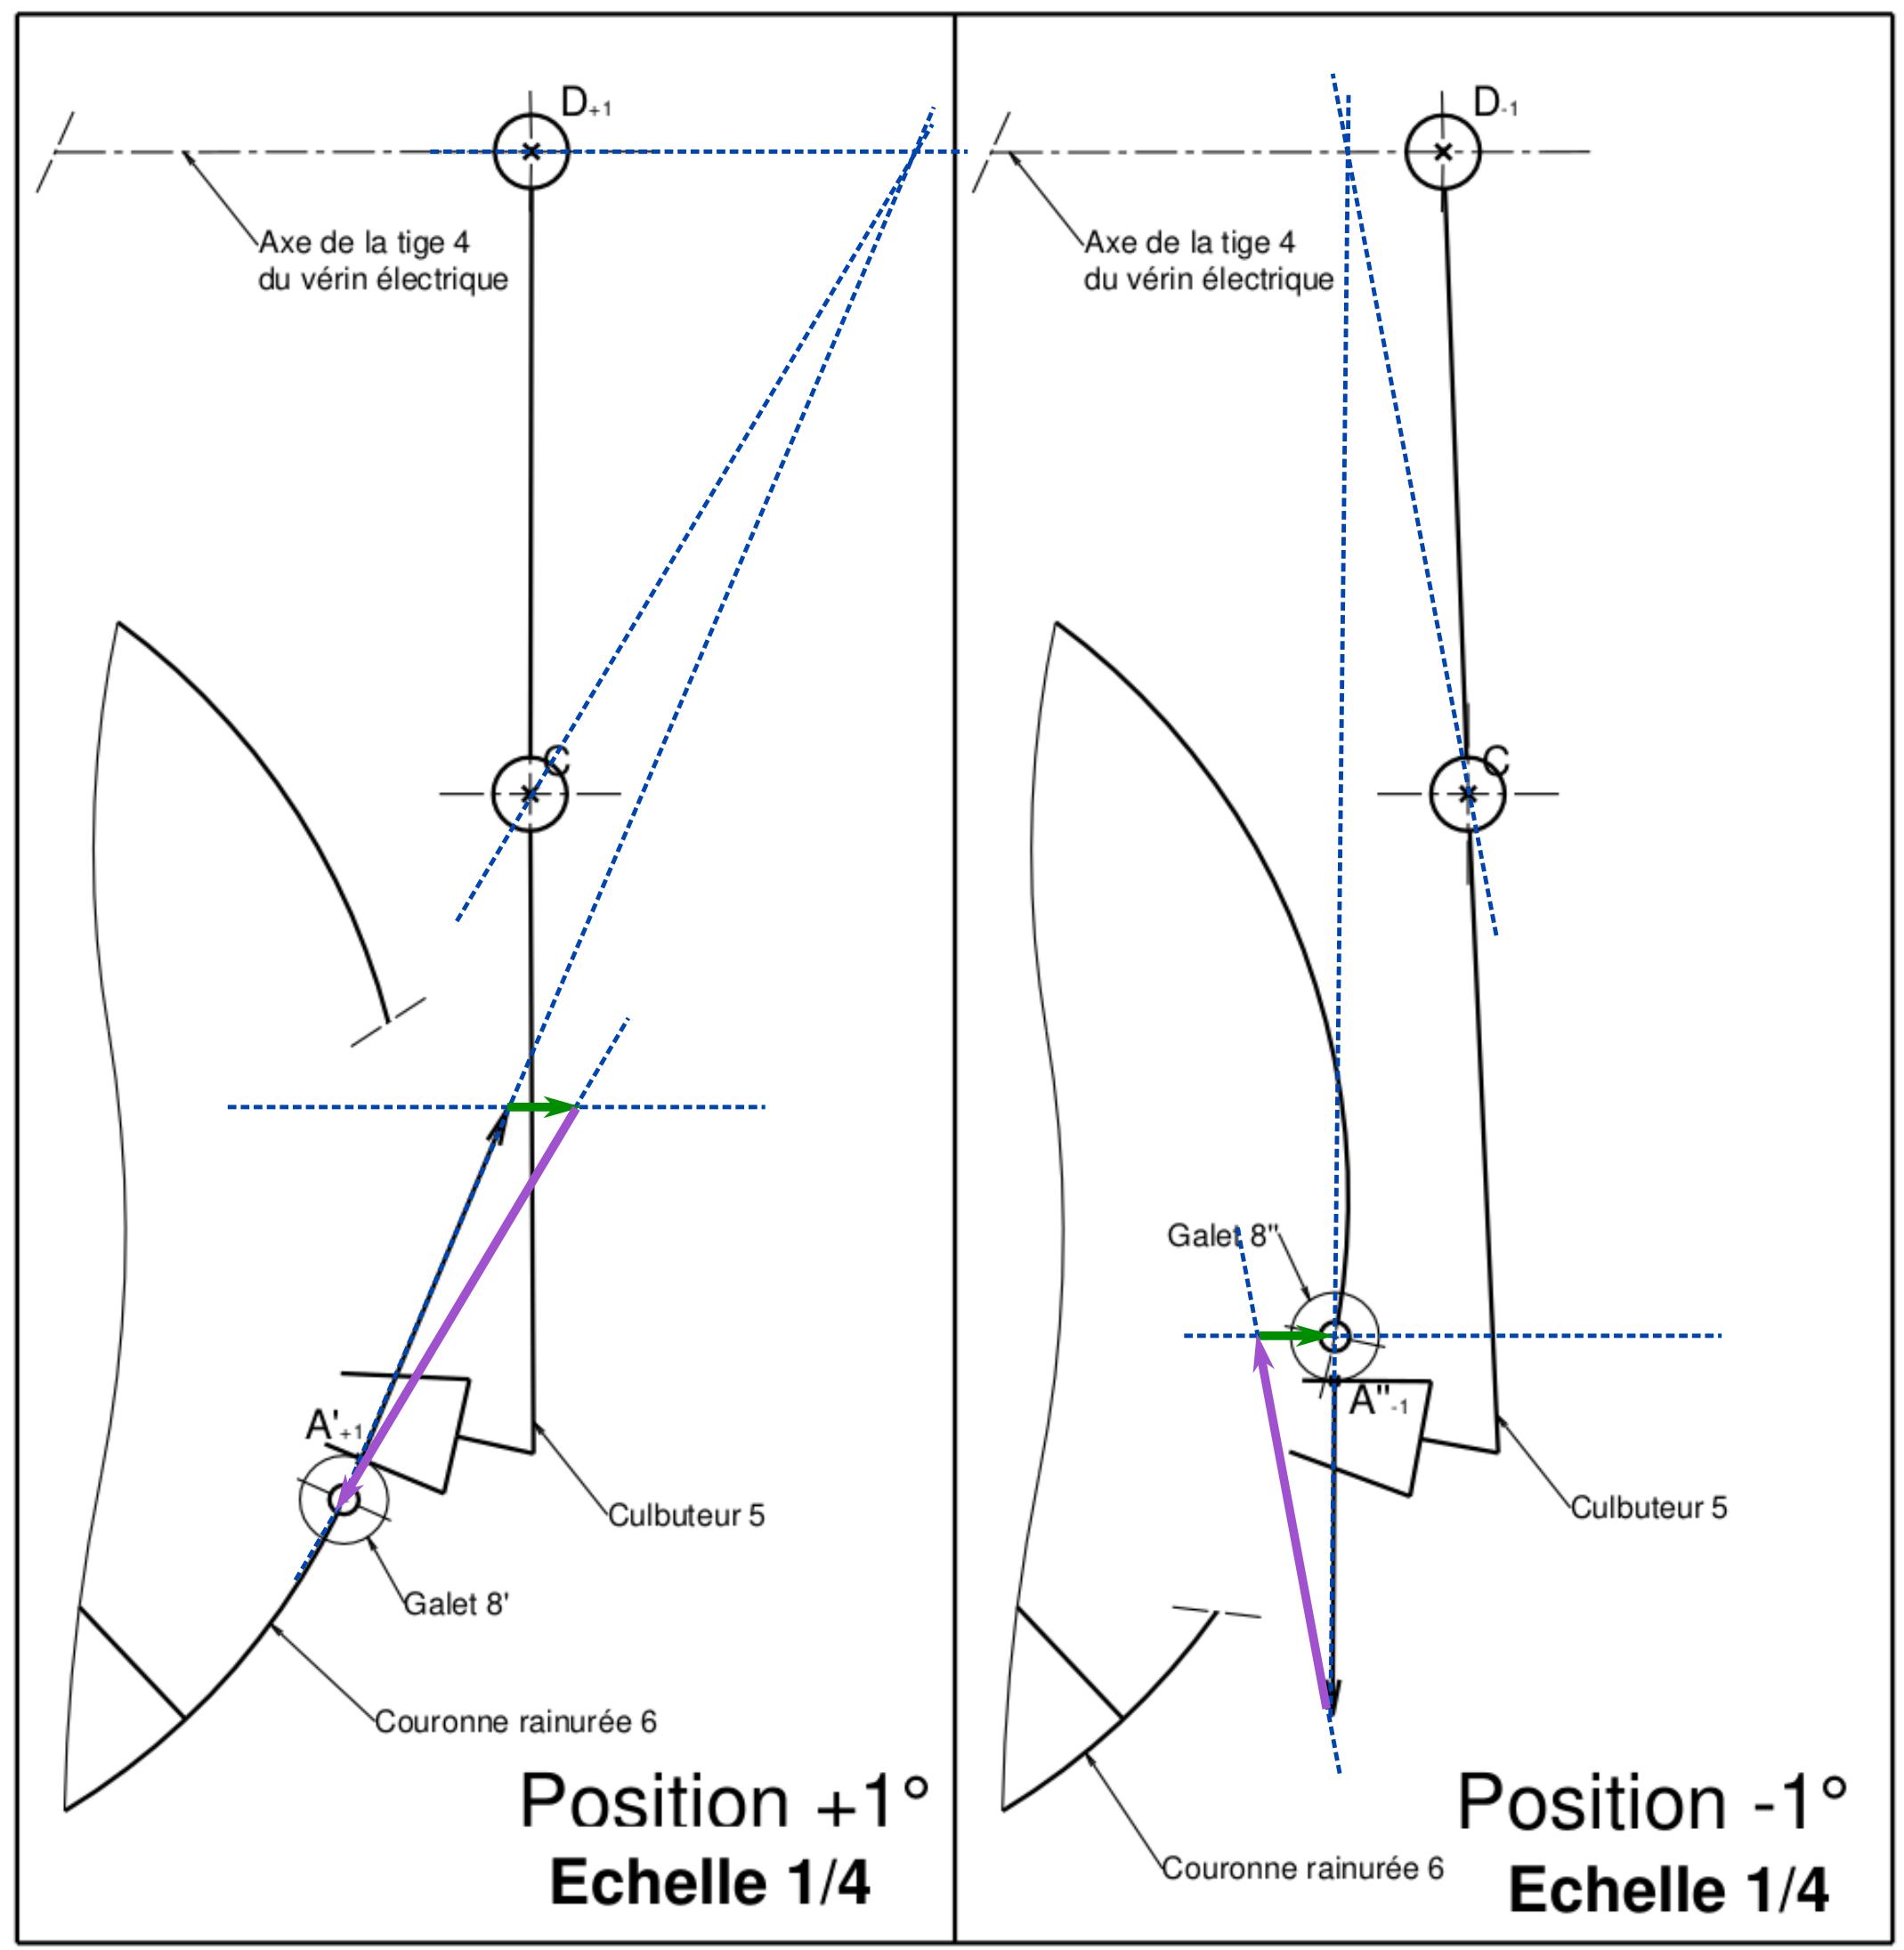
\includegraphics[width=0.9\linewidth]{img/DR04_cor}};
	\draw[lightgray,step=1] (image.south west) grid (image.north east);
	\node at (3,6){$\overrightarrow{A'_{5/8'}}$};
	\node at (5.7,7.2){$\overrightarrow{D_{+14/5}}$};
	\node at (5.2,5){$\overrightarrow{C_{+1bati/5}}$};
	\node at (6.8,14.8){$I_{+1}$};
	\node at (11.4,3){$\overrightarrow{A''_{5/8''}}$};
	\node at (9,5.3){$\overrightarrow{D_{-14/5}}$};
	\node at (9.4,3.5){$\overrightarrow{C_{-1bati/5}}$};
	\node at (10,14.8){$I_{-1}$};
\end{tikzpicture}
\end{center}
}

\reponse{4}{}{
$F_{verin\ max}=\left\|\overrightarrow{D_{4/5}}\right\|\approx \frac{1}{5}\left\|\overrightarrow{A''_{5/8''}}\right\|_{max}\approx 2000N$

Le vérin fonctionne en poussant.
}

\ifdef{\public}{\newpage}

\reponse{0}{\begin{center}
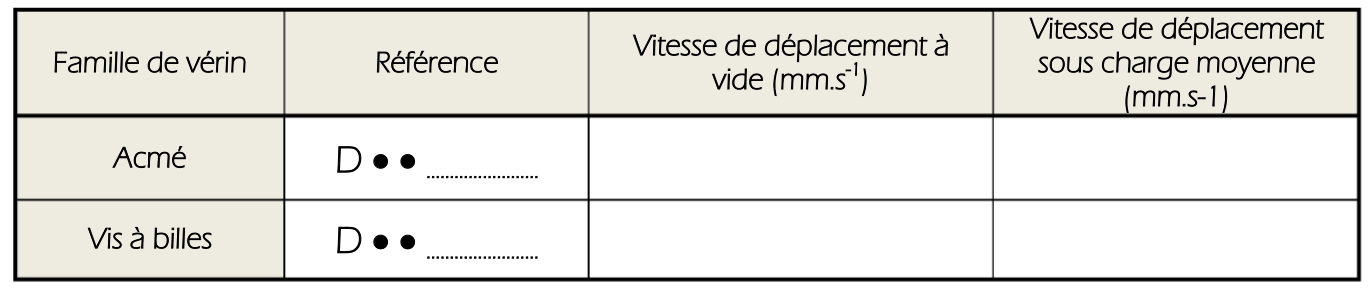
\includegraphics[width=0.8\linewidth]{img/DR05}
\end{center}\vspace{-1cm}}{
\begin{center}
\begin{tikzpicture}

% Include the image in a node
\node [above right,inner sep=0] (image) at (0,0) {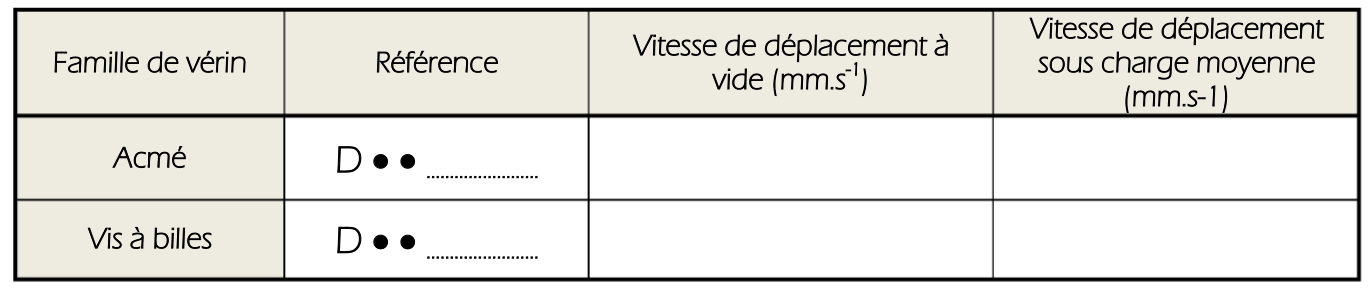
\includegraphics[width=0.9\linewidth]{img/DR05}};
%	\draw[lightgray,step=1] (image.south west) grid (image.north east);
    \node at (5.3,0.6){-05B5};
    \node at (5.3,1.5){-10A5};
    \node at (8.8,0.6){60};
    \node at (8.8,1.5){30};
    \node at (13,0.6){48};
    \node at (13,1.5){23};
\end{tikzpicture}
\end{center}
}

\reponse{4}{}{
$d=\frac{1}{2}\cdot \frac{V_{max}}{\delta}\cdot t^2$
}


\reponse{7}{\begin{center}
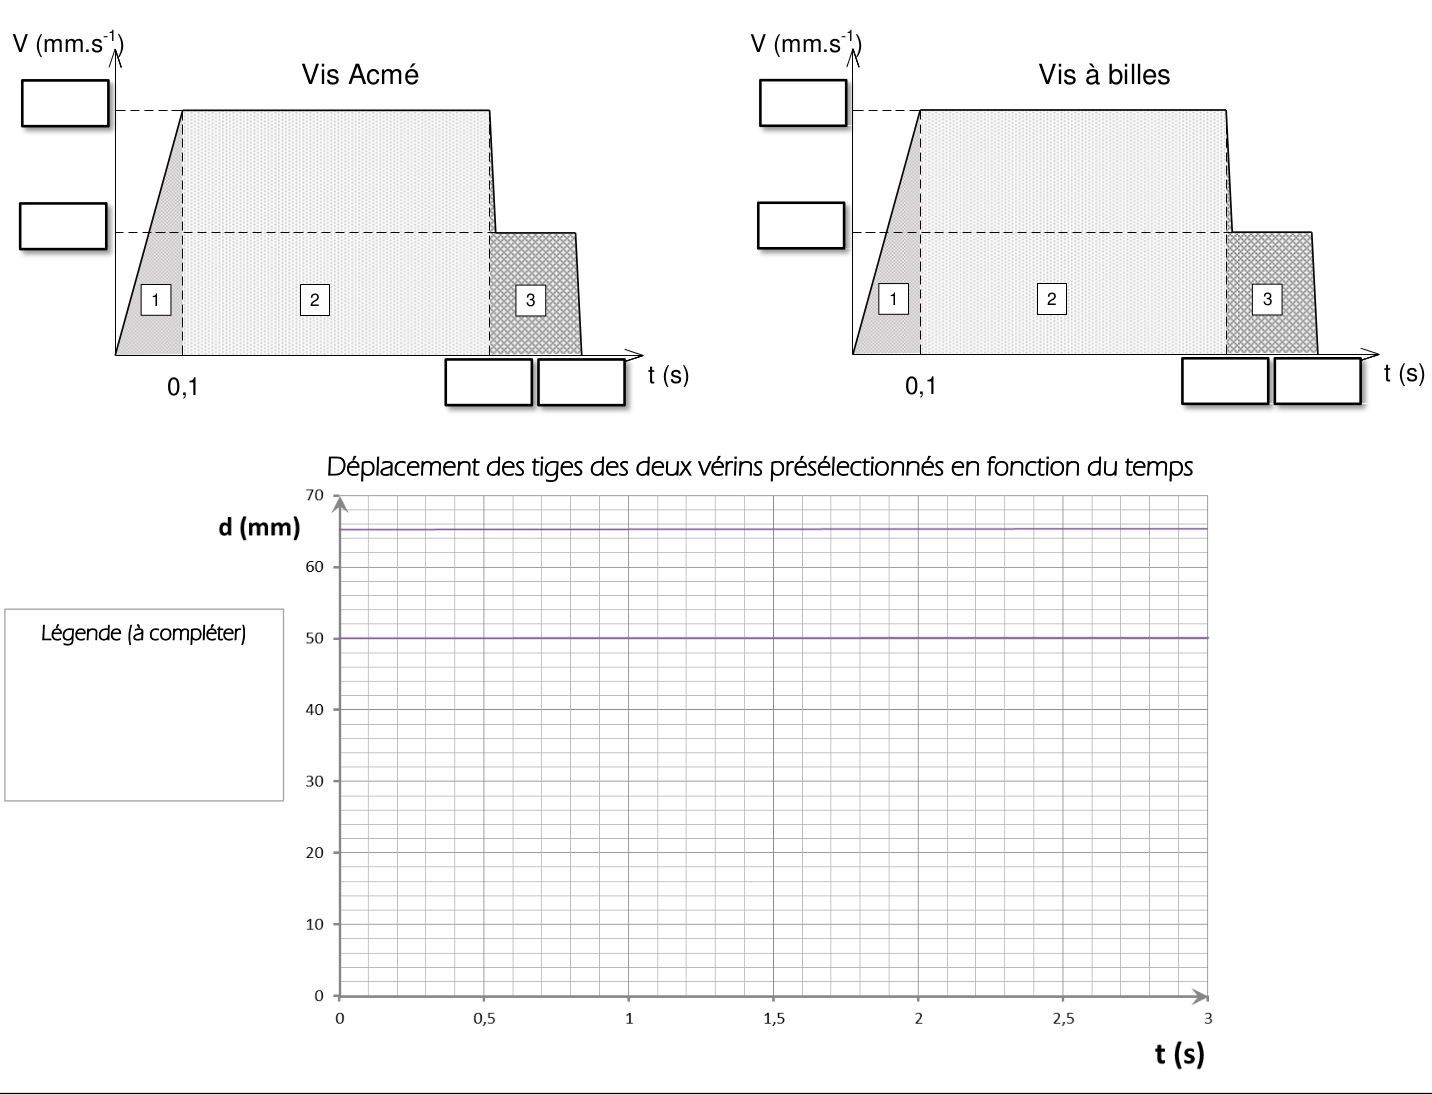
\includegraphics[width=0.8\linewidth]{img/DR06}
\end{center}\vspace{-1cm}}{

On a:
\begin{itemize}
 \item $d_1=\frac{1}{2}\cdot V_{max}\cdot 0,1$,
 \item $d_2=V_{max}\cdot (t_2-0,1)$,
 \item $d_1+d_2=50mm$
 \item $t_2=0,1+\frac{50-d_1}{V_{max}}$
 \item $t_3=t_2+\frac{15}{V_{charge}}$
\end{itemize}

\begin{tabular}{|c|c|c|}
\hline
&Vis acmé & Vis à billes\\
\hline
$d_1$ & $\frac{1}{2}\cdot 30\cdot 0,1=1,5$ & $\frac{1}{2}\cdot 60\cdot 0,1=3$ \\
\hline
$t_2$ & $0,1+\frac{50-1,5}{30}= 0,1+\frac{48,5}{30}\approx 0,1+\frac{48}{30}\approx 1,7$ & $0,1+\frac{50-3}{60}=0,1+\frac{47}{60}\approx 0,1+\frac{48}{60}\approx 0,9$  \\
\hline
$t_3$ & $t_2+\frac{15}{V_{charge}}\approx1,7+\frac{15}{23}\approx1,7+\frac{5}{8}\approx2,325$ & $t_3=t_2+\frac{15}{V_{charge}}\approx 0,9+\frac{15}{48}\approx 0,9+\frac{15}{50}\approx 1,2$ \\
\hline
\end{tabular}
\begin{center}
\begin{tikzpicture}
% Include the image in a node
\node [above right,inner sep=0] (image) at (0,0) {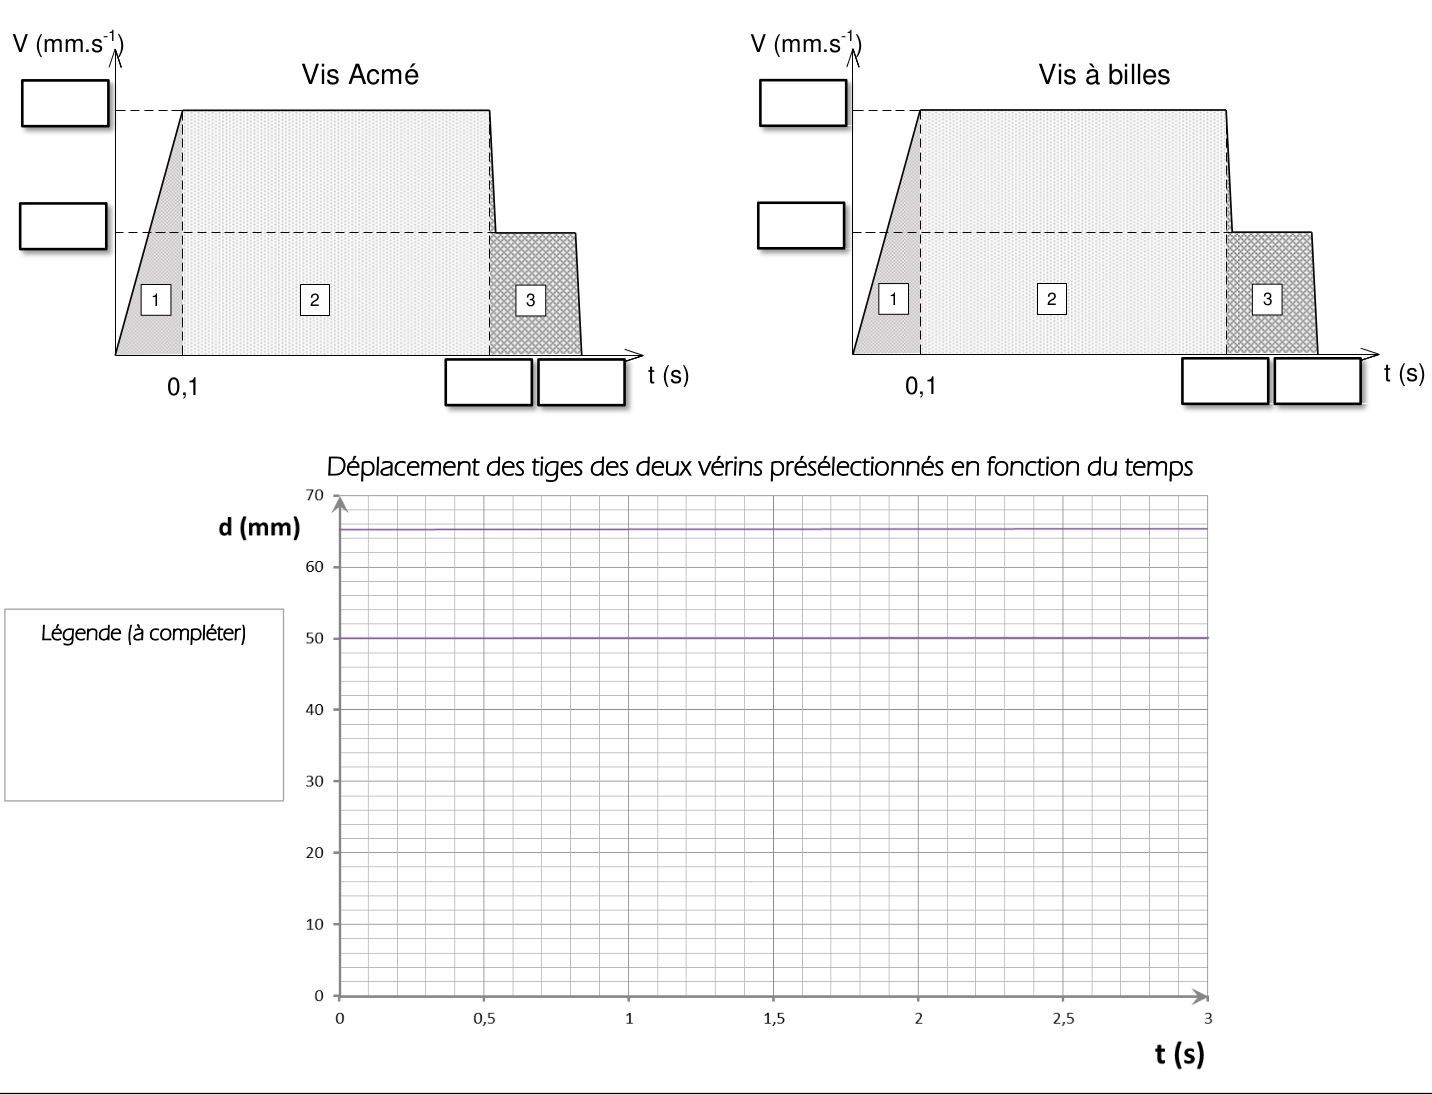
\includegraphics[width=0.9\linewidth]{img/DR06}};
%	\draw[lightgray,step=1] (image.south west) grid (image.north east);
    \node at (0.7,9.25){23};
    \node at (0.7,10.55){30};
    \node at (5.2,7.55){1,7};
    \node at (6.2,7.55){2,3};
    \node at (8.5,9.25){48};
    \node at (8.5,10.55){60};
    \node at (13,7.55){0,9};
    \node at (14,7.55){1,2};
	\draw (3.6,1.05) -- (8.85,4.85);
	\draw (8.85,4.85) -- (10.8,6);
	\draw[dashed] (3.6,1.05) -- (6.4,4.85);
	\draw[dashed] (6.4,4.85) -- (7.3,6);
    \node at (1.5,3.7){Vis à billes};
	\draw[dashed] (0.5,3.4) -- (2.5,3.4);
    \node at (1.5,4.4){Vis Acmé};
	\draw (0.5,4.1) -- (2.5,4.1);
\end{tikzpicture}
\end{center}
}

\reponse{5}{}{
Le vérin à bille Acmé est trop lent, le vérin à billes $D\bullet \bullet-05B5$ convient.
}

\reponse{0}{}{
\begin{center}
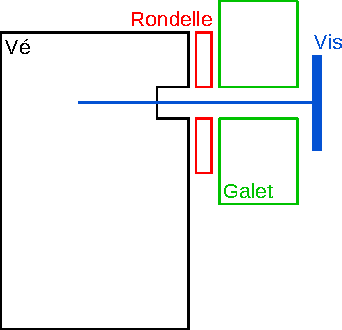
\includegraphics[width=0.4\linewidth]{img/reponse_18}
\end{center}}

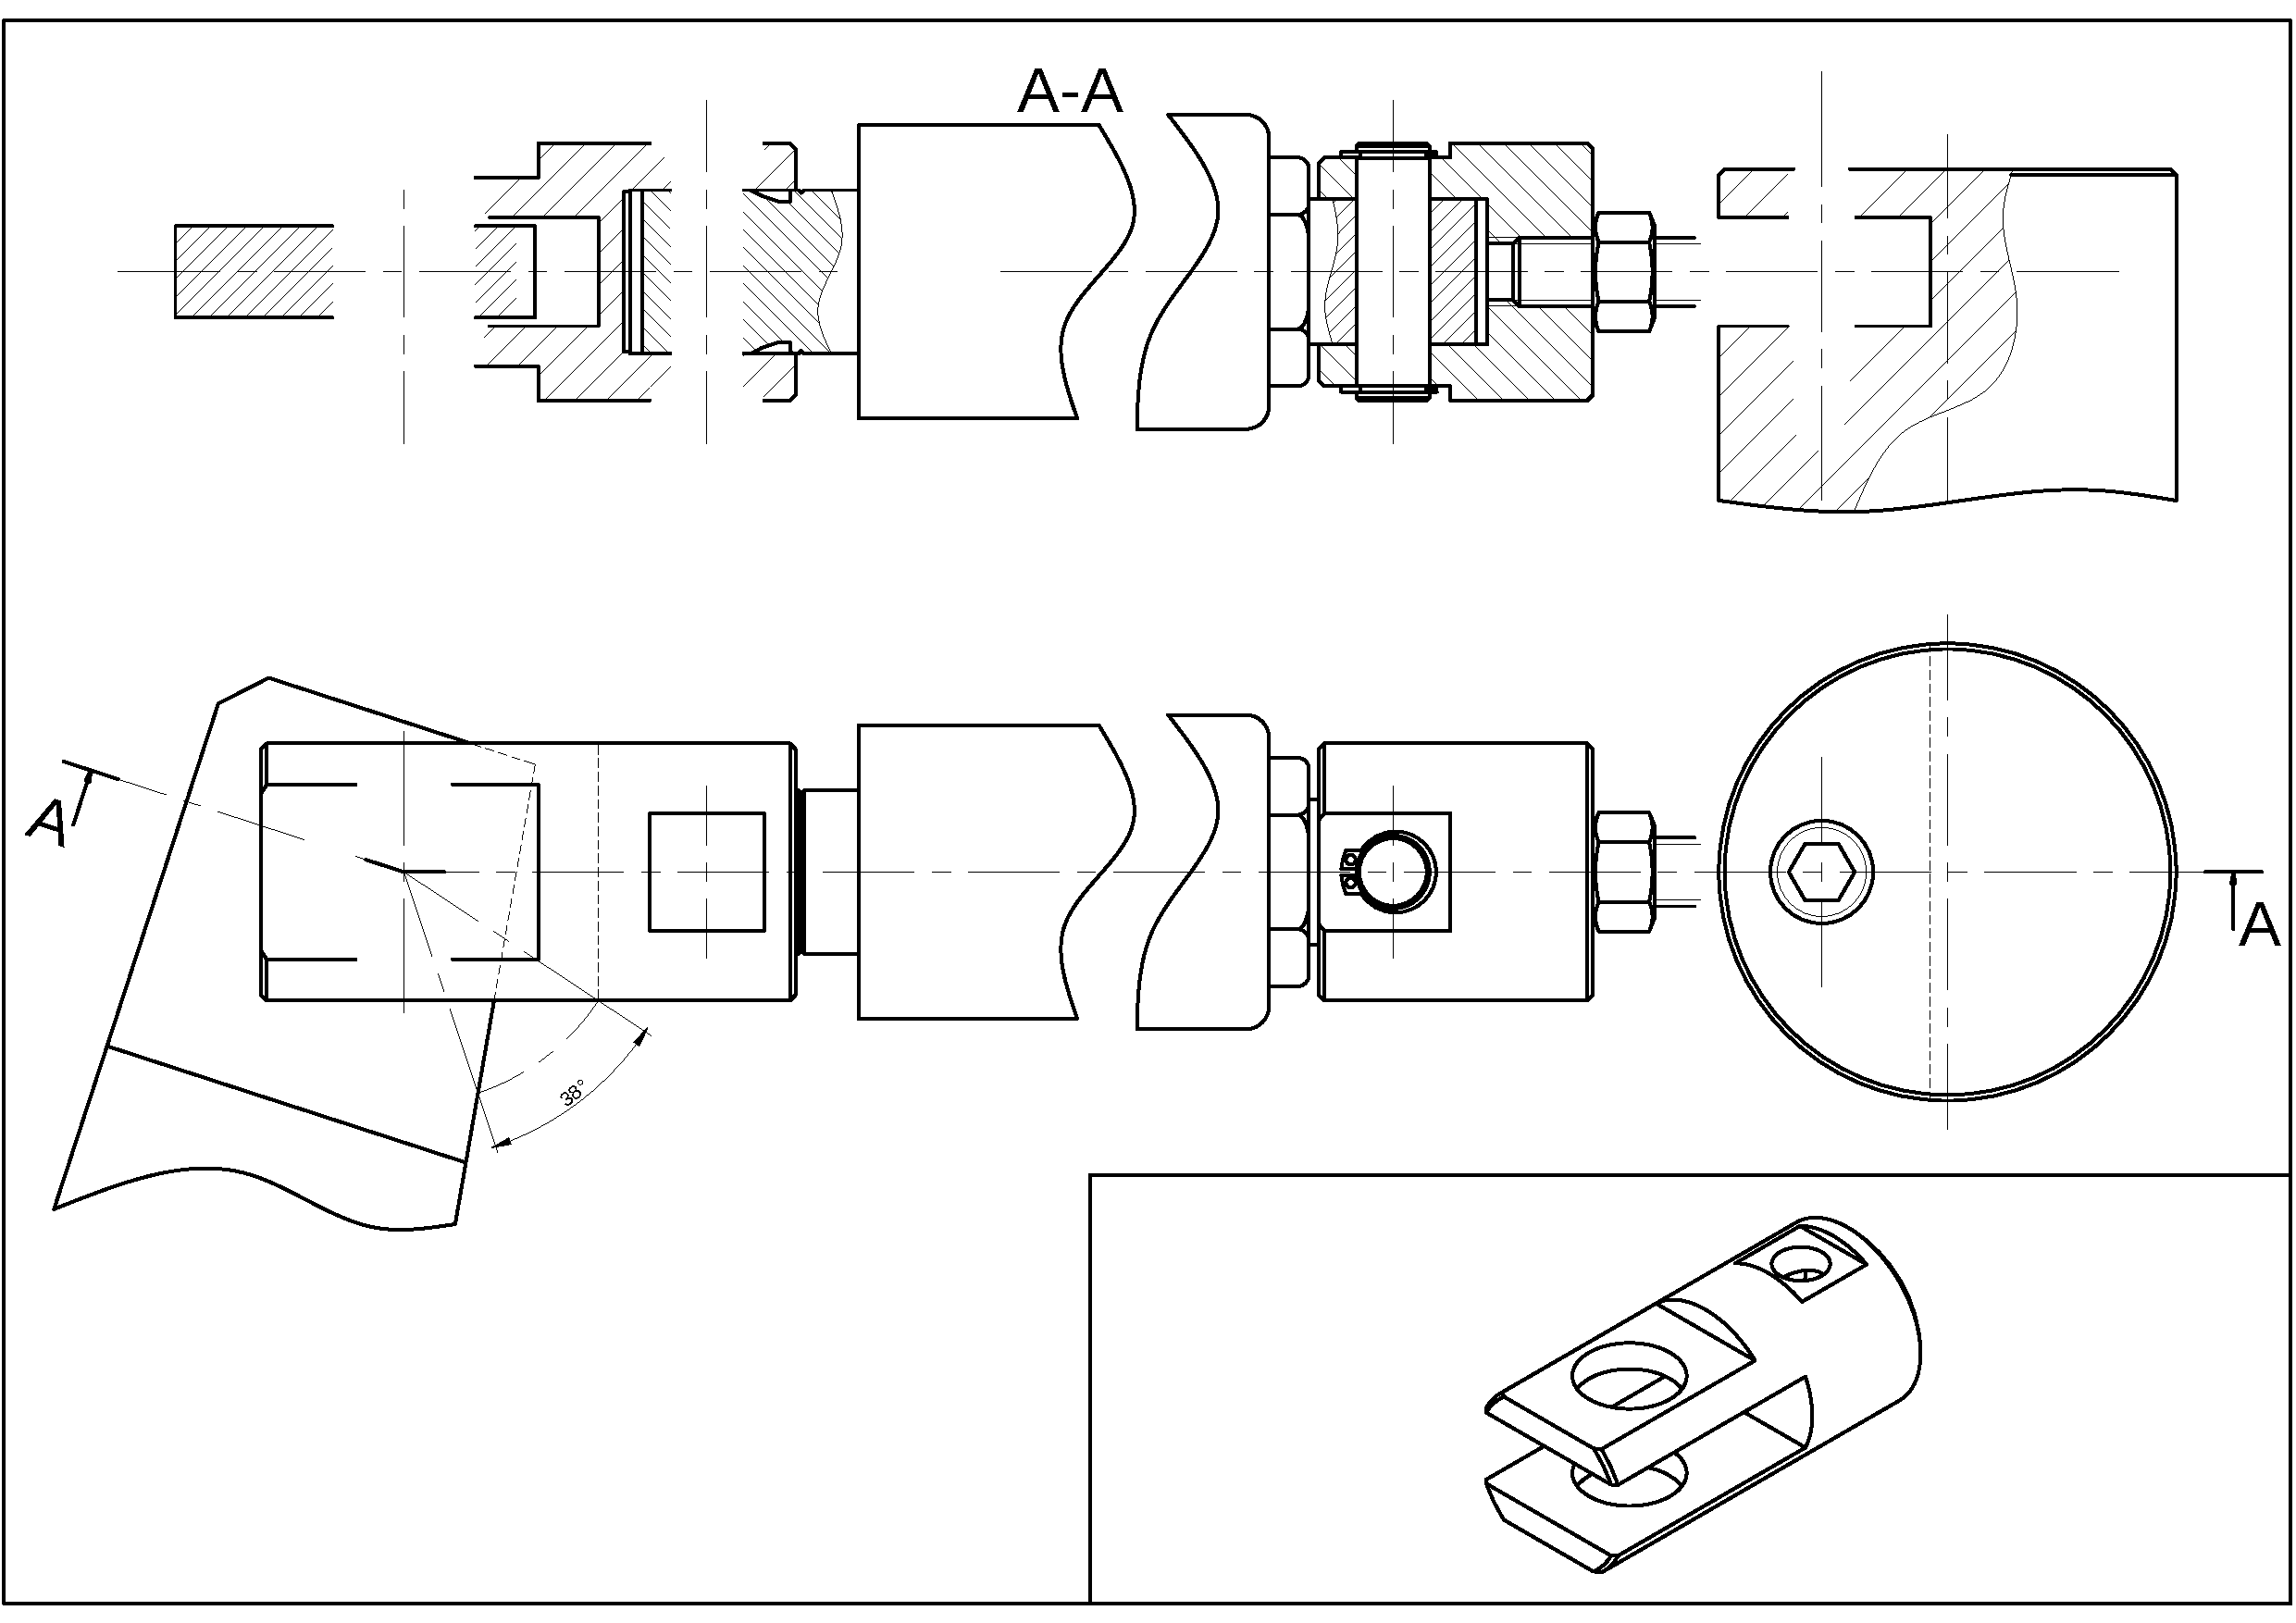
\includepdf[offset=-6mm -6mm,pages=-,angle=90]{img/conception_vierge.pdf}

\end{document}